\chapter{Introduction}
\label{cha:intro}

In this introductory chapter, we will first deal with some preliminaries in Section~\ref{sec:preliminaries},
where will give an overview on the contents of this thesis,
declare the sources these contents are based on,
and present some notational conventions.
In Section~\ref{sec:fundamentals}, we will discuss some basic fundamentals
that frame the work we want to accomplish.
There, we will clarify our notion of statistical inference using parametric models,
and give a brief introduction to the Bayesian approach to statistical inference. %based on the Bayesian paradigm.
Section~\ref{sec:commoncause} then presents a motivating example,
%illustrating the need to go beyond usual Baysian inference
illustrating the advantages in uncertainty modelling that can be gained from using imprecise probability models,
thus serving as a preview on the general concepts we will then introduce in the later chapters.


\section{Preliminaries}
\label{sec:preliminaries}

\subsection{Overview}

In this thesis, a generalisation of Bayesian inference towards the use of imprecise or interval probability is investigated.
A general framework for models based on sets of conjugate priors is established,
and some new models within this framework are proposed.
These models are then compared to some other models based on sets of priors discussed in the literature,
focussing on model behaviour in case of prior-data conflict.

\medskip

With the fundamentals of Bayesian inference based on parametric distributions and conjugate priors
covered in Section~\ref{sec:fundamentals} %\ref{sec:bayes-inference},
a motivating example in Section~\ref{sec:commoncause},
considering the reliability analysis problem of common-cause failure modelling,
serves to show the possibilities of generalised Bayesian inference using sets of conjugate priors.

Chapter~\ref{cha:gbi} then gives a general introduction to the methodology of imprecise probability models,
presenting the general approach to generalised Bayesian inference with lower previsions or sets of priors.
Furthermore, motives for the use of imprecise probability methods are discussed,
among which prior-data conflict (encountered already in the motivating example) and weakly informative priors
are the central topics guiding our assessments of the specific imprecise probability models covered then
in Chapter~\ref{cha:imprecisebayes-conjugate}.

There, we first present a general framework for generalised Bayesian inference using sets of conjugate priors,
giving a superstructure for a number of imprecise probability models
that have been central to the development and application of imprecise probability methods
in statistical inference (Section~\ref{sec:generalmodel}).
Some important favourable inference properties for these models are demonstrated, 
and a range of models that can be subsumed under this framework are discussed with respect to
the handling of prior-data conflict and the possibility to model weak prior information.

Section~\ref{sec:alternatives} briefly discusses some alternative models based on sets of priors,
and compares these to models in the framework from Section~\ref{sec:generalmodel}.
The remainder of Chapter~\ref{cha:imprecisebayes-conjugate}
reproduces two works that suggest novel models %***geared at***
that provide a sophisticated handling of prior-data conflict
(Sections~\ref{sec:jstp} and \ref{sec:isipta11}),
while Section~\ref{sec:luck} gives a short overview on a software implementation.

Chapter~\ref{cha:concluding} concludes the thesis,
giving a summary and discussion of the central achievments,
and sketching some opportunities for applications and avenues for further research.

As supplemental material, the Appendix (Chapter~\ref{cha:appendix}) contains
a study of \pdc\ sensitivity in Bayesian linear regression,
and an informal rationale, together with some first technical results,
for a novel approach that, in addition to prior-data conflict sensitivity,
leads to favourable behaviour in case of strong agreement between prior information and data.



%and illustrates some characteristic modelling opportunities of generalised Bayesian inference, while

%a wealth of favourable model properties

\iffalse
-------------- 2 ---------------------------

After having seen a detailed example for Bayesian inference using sets of conjugate priors in Section~\ref{sec:commoncause},
in this chapter we will now give a general introduction to the methodology of generalised Bayesian inference,
before we give a systematic discussion of models for generalised Bayesian inference with sets of conjugate priors
in the central Section~\ref{sec:generalmodel} of this thesis.

In Section~\ref{sec:ip-intro} below, we will try to outline the general theory of imprecise or interval probability,
describing its main formulations and interpretations, and discuss the generalised Bayesian inference procedure.
Section~\ref{sec:motivation} then gives at first some general motives for the use of imprecise probability methodology,
concluding with the motives especially relevant in the context of the Bayesian approach to statistical inference,
among which prior-data conflict and weakly informative priors will receive special attention
in the model discussion in Chapter~\ref{cha:imprecisebayes-conjugate}.

-------------- 3 ---------------------------

The imprecise probability models based on conjugate priors we will discuss in this chapter
are an important model class,
and have been central to the development and application of imprecise probability methods
in statistical inference.

The chapter is structured as follows.
Section~\ref{sec:generalmodel} attempts to give a systematic overview on these models, %the different models discussed in the literature,
and illustrates some characteristic modelling opportunities of generalised Bayesian inference, while
Section~\ref{sec:alternatives} briefly discusses some alternative models based on sets of priors.
Section~\ref{sec:jstp} then presents one model in detail, namely the so-called
\nymodel\ developed in \textcite{Walter2009a},
and illustrates its application to the Normal-Normal and Dirichlet-Multinomial models. % in more detail. %***JSTP***
Section~\ref{sec:luck} gives a short overview on a software implementation of \nymodel s,
the add-on package \texttt{luck} ***citation*** for the statistical programming environment \textbf{R} \parencite{2013:r}.
Finally,
Section~\ref{sec:isipta11} presents two attempts to further refine inference behaviour in the presence of \pdc.
While the first approach considers more sophisticated shapes for prior parameter sets,
the second is a fundamentally different approach that combining inferences from two arbitrary distinct models.
Interestingly, the inferences from these two approaches in Section~\ref{sec:isipta11} show nevertheless fascinating similarities.

--------------- 4 -----------------------------

We will conclude this thesis with a short summary of, and discussion of the central achievments in, this thesis
in Sections~\ref{sec:concluding-summary} and \ref{sec:concluding-discussion}, respectively.
In Section~\ref{sec:concluding-outlook}, we will sketch some opportunities for applications and avenues for further research.


--------------- A ------------------------------

As supplemental material, the Appendix (Chapter~\ref{cha:appendix}) contains
\begin{enumerate}[(i)]
\item a study of \pdc\ sensitivity in Bayesian linear regression,
presenting a simplified prior model that gives interesting insights into the updating step
for the regression parameters and offers opportunities for inferences based on sets of priors
(Section~\ref{sec:festschrift});
\item some first technical results characterising a new prior parameter set shape,
described informally in Section~\ref{sec:concluding-outlook} below
(Section~\ref{sec:boatshape}).
\end{enumerate}
\fi


\subsection{Sources}


This thesis is partly based on previously published works
where the author of this thesis was the first or second author.
These works, also listed in the Bibliography, are given below.

\printbibliography[heading=none,keyword=disssource]

\iffalse
\begin{itemize}
\item \textcite{Walter2009a}
\item \textcite{Walter2009b} (substantially extended version of \textcite{Walter2010a})
\item \textcite{Walter2011a}
\item \textcite{Walter2012b}
\item \textcite{Troffaes2013a}
\item \textcite{itip-statinf}
\end{itemize}
\fi

In detail, these works have been used in this thesis as described below.

\medskip

In \textbf{Chapter~\ref{cha:intro}},
%Sec.~\ref{sec:stat-inference}: parts of \textcite[\S\S 1.1, 1.2, 1.5]{itip-statinf}
%Sec.~\ref{sec:bayes-inference} uses parts of \textcite[\S\S 1.3, 1.4, 4.1]{itip-statinf},
%except Sec.~\ref{sec:diri-multi}, which is based on \textcite{Walter2012b}.
Section~\ref{sec:fundamentals} is based on \textcite{itip-statinf},
using \S\S 1.1--1.5 and \S 4.1.
Section~\ref{sec:diri-multi}, which is based on \textcite{Walter2012b}.
%
%Sec.~\ref{sec:inferencetasks}: parts of \cite{itip-statinf}
%Sec.~\ref{sec:beta-binom}: parts of \cite{itip-statinf}
%Sec.~\ref{sec:norm-norm}: parts of \cite{itip-statinf}
%
Section~\ref{sec:commoncause} is based on %parts of
\textcite{Troffaes2013a},
%where in particular Sec.~\ref{sec:basic-param-model} and Sec.~\ref{sec:alpha-factor-model}
%have been written primarily by Matthias Troffaes.
except Section~\ref{sec:commoncause-motivation}, which was newly written for this thesis.
%Sec.~\ref{sec:alpha-factor-prior}: parts of \cite{Troffaes2013a}

\medskip

In \textbf{Chapter~\ref{cha:gbi}},
Section~\ref{sec:ip-intro} was newly written for this thesis,
except Section~\ref{sec:imprecisebayes}, which is based on \textcite[\S 4.2]{itip-statinf},
and Section~\ref{sec:updating}, which is based on parts of \textcite[\S 4.4]{itip-statinf}.
%where the latter was mainly written by Thomas Augustin.
Also, Section~\ref{sec:ip-related} uses parts of \textcite[\S 5.2]{itip-statinf} and \textcite[\S 6.1]{itip-statinf}.
%
Sec.~\ref{sec:motivation} was newly devised for this thesis,
under use of \textcite[\S 2.3]{itip-statinf}
for the last paragraph in Sec.~\ref{sec:motivation:bayesian-foundational},
and Sections~\ref{sec:motivation:near-ignorance} and \ref{sec:motivation:pdc}.
%
Section~\ref{sec:ip-alternatives} uses parts of \textcite[\S 2.2, 2.4]{itip-statinf},
and a paragraph from \textcite[\S 7]{itip-statinf}.

\medskip

In \textbf{Chapter~\ref{cha:imprecisebayes-conjugate}},
Section~\ref{sec:generalmodel} is based on \textcite[\S 4.3]{itip-statinf}.
%which was written primarily by Gero Walter.****
Section~\ref{sec:alternatives} was newly written for this thesis,
using some very minor parts of \textcite[\S 4.2, \S 4.4]{itip-statinf}.
Section~\ref{sec:jstp} is a slightly abriged reproduction of \textcite{Walter2009a},
with a minor change of notation towards the one introduced in Section~\ref{sec:regularconjugates}
(most importantly, writing $\nn$ and $\yn$ for the canonical posterior parameters
instead of $n^{(1)}$ and $y^{(1)}$, respectively).
%This paper was the result of a collaborative work, where both authors contributed
%more or less in equal parts. While Gero Walter contributed central concepts and basic ideas,
%along with the theoretical results, Thomas Augustin devised most of the structure,
%and contributed most of the introductory and concluding sections.***
%
Section~\ref{sec:luck} gives a short overview on a software implementation
of the model presented in Section~\ref{sec:jstp}.
Author and maintainer of this add-on package \texttt{luck}***citation*** is Gero Walter,
with Norbert Krautenbacher as a second author, who contributed code for an application
to exponentially distributed data.
%
Section~\ref{sec:isipta11} consists of \textcite{Walter2011a},
again with a slight change of notation for consistency with the rest of the material presented in this thesis.
Specifically, the success probability in Bernoulli trials is denoted by $\theta$ instead of $p$.
%All three authors worked collaboratively on the work as whole but with emphasis on different parts.
%Section~\ref{sec:ibbm} was devised and written primarily by Gero Walter,
%while Section~\ref{sec:weightedinf} was devised and written primarily by Frank Coolen.
Here, it was possible to add a few explanatory paragraphs
that could not appear in the original publication due to page restrictions. 
%Thomas Augustin contributed substantially to all parts of the manuscript,
%especially in the introductory and concluding sections.***

\medskip

\textbf{Chapter~\ref{cha:concluding}} was newly written for this thesis.

\medskip

In the \textbf{Appendix} (Chapter~\ref{cha:appendix}),
Section~\ref{sec:festschrift} consists of \textcite{Walter2009b},
which is a substantially extended version of \textcite{Walter2010a},
reproduced here with a slight change in notation and some added comments.
%In this work, the result of a collaborative effort, Gero Walter contributed 
%the description of the examples in Section~\ref{sec:iid},
%and the computations and most of the write-up in Sections~\ref{sec:scp} and \ref{sec:cccp}.
%Sections~\ref{sec:festschrift-intro} and \ref{sec:discussion-festschrift} were a joined effort
%of Gero Walter and Thomas Augustin.
%
Section~\ref{sec:boatshape} was instead written newly for this thesis.


\subsection{Notation}
\label{sec:notation}

Scalars are denoted by italic letters ($x$, $\theta$),
whereas vectors are denoted by bold italic letters ($\vec{x}$, $\btheta$).
Matrices are written in bold regular (i.e., non-italic) uppercase letters, like $\mbf{X}$, $\mbf{Z}$,
and transposed matrices are marked by a raised uppercase sans serif `T' ($\mbf{X}^\tra$).
The trace of a matrix is denoted by $\tr(\mbf{X})$;
unit or identity matrices are denoted by $\mbf{I}$,
sometimes with an added subscript indicating their size
(in the case that the size may be not obvious or in order to emphasise it),
such that $\mbf{I}_p$ denotes a unit matrix of size $p \times p$.

For statistical models, samples, i.e.\ realisations of random variables,
are denoted by lowercase letters ($x$, $\x$),
random quantities by uppercase letters ($X$, $\vec{X}$);
however, as this thesis is mostly concerned with Bayesian methods,
the strict distrinction between random variables and `fixed' quantities as made in frequentist statistics
is not maintained throughout most of the thesis.

Sets or spaces are given as calligraphic uppercase letters ($\mathcal{X}$, $\Y$, $\mathcal{M}$).
Some special sets are denoted as follows:
the real numbers by $\reals$, positive real numbers by $\posreals$,
nonnegative real numbers by $\posrealszero$,
and the space of $q$-dimensional tuples of real numbers by $\reals^q$.

In the Bayesian setting, prior and posterior probability distribution functions, i.e.\ densities on parameters,
are usually denoted by lowercase letter $p$;
sample model densities (probability distribution functions on observable quantities)
are denoted by lowercase letter $f$:
$f(x)$, $p(\theta)$.

This distinction for densities on parameters or samples
is not maintained for the associated probability measures and cumulative distribution functions:
cumulative distribution functions are denoted by uppercase letter $\cdf$,
e.g., $\cdf(x) := \int_{-\infty}^x f(u) \dd u$, or $\cdf(\theta) := \int_{-\infty}^\theta f(\psi) \dd \psi$;
probability measures, e.g.\ for subsets $A$ of a sample space $\Omega$,
or a subset $\Theta_1$ of the parameter space $\Theta$,
are denoted by uppercase $\p$,
i.e.\ $\p(A) = \sum_{\omega \in A} f(\omega)$ if $\Omega$ is countable,
or $\p(\Theta_1) = \int_{\Theta_1} p(\theta) \dd \theta$ for continuous $\Theta$.

Expectation and variance of a random quantity $X$ are denoted by $\E[X]$ and $\V(X)$, respectively.
In a Bayesian setting, quantities identifying the distribution
(with respect to which expectation and variance are calculated)
are added in the argument, seperated by a vertical line, as in $f(x\mid\theta)$, or $\E[\theta\mid\nz, \yz]$.
%(This notation refers to the auffassung in Bayesian statistics that ****)

Other notational conventions are declared upon introduction of the concepts they are representing.

\newpage

\section{Some Fundamentals}
\label{sec:fundamentals}

In this section, we will briefly introduce our notion of statistical inference,
%first give a brief introduction to statistical inference
and discuss models that are used to describe random samples.
Then, we will give a short introduction into the basic principles of Bayesian inference
based on conjugate priors.


\subsection{Statistical Inference}
\label{sec:stat-inference}

Statistical inference is about learning from data.
It is basically concerned with inductive reasoning,
i.e., establishing a general rule from observations.
As is long known as the problem of induction \parencite{1739:hume},
it is impossible to justify inductive reasoning by pure reason,
and therefore one cannot infer general statements (laws) with absolute truth from single observations.
%***statistical models are built for a certain purpose. (citexxx George P. Box, Kaplan?)\\
%***models try to mirror certain aspects of reality: those deemed relevant to answer %the question(s) at hand etc.
The statistical remedy for this inevitable and fundamental dilemma of any type of inductive reasoning is
(postulated, maybe virtual) \emph{randomness} of the sampling process that generates the data.
If, and only if, the sample is, or can be understood as, drawn randomly,
probability theory allows to quantify the error of statistical propositions concluded from the sample.

Specifically, to model the randomness, a \emph{statistical model} is formulated.
It is a tuple $(\mathcal{X}, \mathcal{Q})$, consisting of the \emph{sample space} $\mathcal{X}$,
i.e.\ the domain of the random quantity $X$ under consideration,
and a set $\mathcal{Q}$ of probability distributions,%
\footnote{Most models of statistical inference rely on $\sigma$-additive probability distributions.
Therefore, technically, in addition an appropriate ($\sigma$-)field $\sigma(\mathcal{X})$,
describing the domain of the underlying probability measure, has to be specified.
In most applications there are straightforward canonical choices for $\sigma(\mathcal{X})$,
and thus $\sigma$-fields are not explicitly discussed here.}
collecting all probability distributions that are judged to be potential candidates for the distribution of $X$.
In this setting $\mathcal{Q}$ is called \emph{sampling model} and every element $\p\in \mathcal{Q}$ \emph{(potential) sampling distribution}.
The inferential task is to learn the true element $\p^* \in \mathcal{Q}$ from multiple observations of the random process producing $X$.


\subsection{Parametric Models}
\label{sec:parametricmodels}

In this thesis, generally, so-called \emph{parameteric models} are considered,
where $\mathcal{Q}$ is pa\-ra\-me\-trised by a parameter $\vartheta$ of finite dimension,
assuming values in the so-called \emph{parameter space} $\Theta$, $\Theta \subseteq \reals^q, \ q < \infty$,
i.e.\ ${\cal Q}=\left(\p_\vartheta\right)_{\vartheta \in \Theta}$.
Here, the different sampling distributions $\p_\vartheta$ are implicitly understood as belonging to a specific class of distributions,
the basic type of which is assumed to be known completely
(e.g., normal distributions, see Example~\ref{ex:normaldist} below), %as in Section~\ref{sec:normaldist} below),
and only some characteristics $\vartheta$ (e.g., the mean) of the distributions are unknown.

Throughout, we will assume (as is the case for all common applications)
that the underlying candidate distributions $\p_\vartheta$ of the random quantity $X$
are either discrete or absolutely continuous with respect to the Lebesgue measure
\parencite[see, e.g., ][pp.~32f, 38 for some technical details]{1993:karr} for every $\vartheta \in \Theta$.
Then it is convenient to express every $\p_\vartheta$ in the discrete case by its \emph{mass function} $f_\vartheta$,
with $f_\vartheta(x):=\p_\vartheta(X=x),\forall x \in \mathcal{X}$,
and in the continuous case by its \emph{probability density function} (pdf) $f_\vartheta$,
where $f_\vartheta$ is such that $\p_\vartheta(X \in [a,b]) = \int_a^b f_\vartheta(x) \dd x$.

An \emph{i.i.d.\ sample of size} $n$ (where \emph{i.i.d.}\ abbreviates independent, identically distributed)
\emph{based on the parametric statistical model} %
$(\mathcal{X}, (p_\vartheta)_{\vartheta \in \Theta})$ is a vector
\[
\vec{X} = (X_1, \ldots, X_n)^\tra %\label{120722-1}
\]
of independent random quantities $X_i$ with the same distribution $\p_\vartheta$.
Then $\vec{X}$ is defined on $\mathcal{X}^n$ with probability distribution $\p_\vartheta^{\otimes n}$
as the $n$-dimensional product measure describing the independent observations.
For Bayesian approaches as discussed here,
independence is often replaced by exchangeability \parencite[see, e.g.,][\S 4.2]{2000:bernardosmith}.
$\p_\vartheta^{\otimes n}$ thus has the probability mass or density function
\[
f_\vartheta(x_1, \ldots, x_n) := \prod_{i=1}^{n} f_\vartheta(x_i)\,.%\label{120710-2}
\]
The term \emph{sample} is then also used for the concretely observed value(s) $\x=(x_1, \ldots, x_n)^\tra$.%
%\footnote{Throughout, random quantities are denoted by capital letters, their values, or realizations, by small letters.}

\medskip

%In Sections~\ref{sec:normaldist} and \ref{sec:multinomdist},
Now
we will present two examples for basic parametric models that will be repeatedly discussed further on.


%\subsection{The Normal Distribution}
%\label{sec:normaldist}
\begin{example}[Normal distribution]
\label{ex:normaldist}

A common model for observations that in principle can assume any value on the real line
is the \emph{normal distribution} with parameters $\mu$ and $\sigma^2$, also called the \emph{Gaussian distribution}.
Typical examples for data of this kind are scores in intelligence testing, or technical measurements in general.%
\footnote{The normal distribution is distinguished by the central limit theorem
(see, e.g., \cite[\S 7.3]{1993:karr}, or \cite[\S 9]{1968:breiman}), stating that, under regularity conditions,
the distribution of an appropriately scaled sum of $n$ standardized random variables converges to a normal distribution
for $n \to \infty$.}

For each observation $x_i$, $i=1,\ldots, n$, the normal probability density is
\begin{align*}
f_{(\mu, \sigma^2)}(x_{i}) &= \frac{1}{\sqrt{2\pi\sigma^2}}\exp\Big\{ -\frac{1}{2\sigma^2}(x_{i} - \mu)^2 \Big\}\,,
\end{align*}
with the two parameters $\mu \in \reals$ and $\sigma^2 \in \reals_{>0}$
being in fact the mean and the variance of (the distribution of) $x_i$, respectively.
As a shortcut, we write $x_i \sim \norm(\mu, \sigma^2)$.
%a normal density with $\mu=0$ and $\sigma^2=1$ is displayed
%in Figure~\ref{inference:fig:normal-vs-cauchy}, page~\pageref{inference:fig:normal-vs-cauchy}.

With the independence assumption, the density of $\x = (x_1,\ldots,x_n)$ amounts to
\begin{align}\label{eq:normaldens}
f_{(\mu, \sigma^2)}(\x)
 &= \prod_{i=1}^n f_{(\mu, \sigma^2)}(x_{i})
  = (2\pi\sigma^2)^{-\frac{n}{2}}\exp\Big\{ -\frac{1}{2\sigma^2}\sum_{i=1}^n (x_{i} - \mu)^2 \Big\}\,.
\end{align}
Later on, we restrict considerations to the case where the variance is known to be equal to $\sigma_0^2$,
denoted by $x_i \sim \norm(\mu, \sigma_0^2)$.
Inference may thus concern the parameter $\mu$ directly,
or future observations $x_{n+1}, x_{n+2}, \ldots$ in a chain of i.i.d.\ observations.
\end{example}


%\subsection{The Multinomial Distribution}
%\label{sec:multinomdist}
\begin{example}[Multinomial distribution]
\label{ex:multinomdist}

The \emph{multinomial distribution} is a common model for samples where only a limited number of distinct values can be observed.
%like in the data from an election poll, or from a pharmacological study asking about a certain set of adverse reactions.
These distinct values are often named \emph{categories} (hence the term \emph{categorical data}),
and are usually numbered from $1$ to $k$, without imposing any natural ordering on these values.
We have therefore a discrete distribution,
giving the probability for observing certain category counts $(n_1, \ldots, n_k) = \vec{n}$ in a sample of $n$ observations in total.
Thus, $\sum_{j=1}^k n_j = n$.

We start the definition of the multinomial distribution by decomposing the collection of $n$ observations into its constituents,
single observations of either of the categories $1,\ldots,k$.
Such a single observation, often named \emph{multivariate Bernoulli observation}, can be encoded as a vector $\x_i$ of length $k$,
where the $j$-th element, $x_{ij}$, equals $1$ if category $j$ has been observed, and all other elements being $0$.
Given the vectorial parameter $\btheta$ of length $k$,
where the component $\theta_j$ models the probability of observing category $j$ in a single draw
(therefore $\sum_{j=1}^k \theta_j = 1$),
the probability for observing $\x_i$ can be written as
\begin{align*}
f_{\btheta}(\x_i) = \prod_{j=1}^k \theta_j^{x_{ij}}\,.
\end{align*}
Assuming independence, the probability for observing a certain sequence
$\mbf{x} = (\x_1, \ldots, \x_n)$ of $n$ observations can thus be written as
\begin{align*}
f_{\btheta}(\mbf{x}) &= \prod_{i=1}^n f_{\btheta}(\x_i)
                \propto \prod_{i=1}^n \prod_{j=1}^k \theta_j^{x_{ij}}
                      = \prod_{j=1}^k \theta_j^{\sum_{i=1}^n x_{ij}}
                      = \prod_{j=1}^k \theta_j^{n_j}\,,
\end{align*}
where $n_j = \sum_{i=1}^n x_{ij}$ tells us how often category $j$ was observed in the sample.

For the probability to observe a certain category count $(n_1, \ldots, n_k) = \vec{n}$,
we have to account for the different possible orderings in $\mbf{x}$ leading to the same count vector $\vec{n}$.
Therefore,
\begin{align}\label{eq:multinomdens}
f_{\btheta}(\vec{n}) &= \binom{n}{n_1,\ldots,n_k} \prod_{j=1}^k \theta_j^{n_j}
                      = \frac{n!}{n_1!\cdot \ldots \cdot n_k!} \prod_{j=1}^k \theta_j^{n_j}\,.
%               \propto \prod_{j=1}^k \theta_j^{n_j}\,.
\end{align}
As a shortcut, we write $\vec{n} \sim \mult(\btheta)$.
\end{example}


\subsection{Statistical Inference with the Bayesian Paradigm}
\label{sec:bayes-inference}

As the inference models discussed in this thesis are all based on the Bayesian approach to statistical inference,
we will now give a short introduction to the basic principles of Bayesian inference.

\medskip

The Bayesian approach requires (possibly subjective) knowledge on the parameter $\vartheta$ to be expressed by a probability distribution on%
\footnote{Again we implicitly assume that $\Theta$ is complemented by an appropriate $\sigma$-field $\sigma(\Theta)$.}
$\Theta$, with the probability mass or density function $p(\vartheta)$ called \emph{prior distribution}.
Indeed, the basic assumption in the Bayesian approach is that \emph{any} prior information about $\Theta$
can be sufficiently expressed by a (precise) prior $p(\theta)$.%
\footnote{This assumption is refuted most prominently by \textcite{1991:walley},
whose theory of Bayesian inference without a need for precise priors will be discussed in Section~\ref{sec:ip-intro}.}
Interpreting the elements $f_\vartheta(\x)$ of the sampling model as conditional distributions of the sample given the parameter,
denoted by $f(\x\mid\vartheta)$ and called \emph{likelihood},
turns the problem of statistical inference into a problem of probabilistic deduction,
where the \emph{posterior distribution}, i.e.\ the distribution of the parameter given the sample data,
can be calculated by Bayes' Rule.%
\footnote{\citeauthor{1987:gillies} \parentext{\citeyear{1987:gillies}, \citeyear{2000:gillies}} argues
that Bayes' Theorem was in fact developed in order to confront the problem of induction as posed by \textcite{1739:hume}.}
Thus, in the light of the sample $\x= (x_1, \ldots, x_n)$, the prior distribution is updated by Bayes' Rule
to obtain the posterior distribution with density or mass function
\begin{align}
\label{eq:bayesrule}
p(\vartheta\mid\x) \propto f(\x\mid\vartheta) \cdot p(\vartheta)\,.
\end{align}
The posterior distribution is understood as comprising all the information from the sample and the prior knowledge.
It therefore underlies all further inferences on the parameter $\vartheta$,
like point estimators, interval estimators,
or the \emph{posterior predictive distribution},
which is the distribution of further observations based on $p(\vartheta\mid\x)$
(see Eq.~\eqref{eq:posteriorpredictive} below).


\subsubsection{Regular Conjugate Families of Distributions}
\label{sec:regularconjugates}

Traditional Bayesian inference is frequently based on so-called \emph{conjugate priors} related to a specific likelihood.
Such priors have the convenient property that the posterior resulting from~\eqref{eq:bayesrule}
belongs to the same class of parametric distributions as the prior, and thus only the parameters have to be updated,
which makes calculation of the posterior and thus the whole Bayesian inference easily tractable.%
\footnote{This motivation for the use of conjugate priors can be founded on formal arguments.
As will be explained below, the posterior expectation of the parameter of interest
is actually a linear function of a sufficient statistic of the data and the prior expectation.
It turns out that, under some regularity conditions, requiring such linearity of posterior expectation
implies the use of conjugate priors \parencite[p.~276]{2000:bernardosmith}.}
% comment Frank: exponential family was known in pre-Bayes days as Kap***-Dar**** family

Fortunately, there are general results guiding the construction of conjugate priors in several models used most frequently in practice,
namely in the case where the sample distribution belongs to a so-called \emph{(regular) canonical exponential family}
\parencite[e.g.,][pp.~202 and 272f]{2000:bernardosmith}. %Def.~4.12 and Prop.~5.6
This indeed covers many sample distributions relevant in a statistician's everyday life,
like Normal and Multinomial models, Poisson models, or Exponential and Gamma models.
After presentation of the general framework, we will discuss its instantiation for the Normal
and the Multinomial sampling models as introduced
in Examples~\ref{ex:normaldist} and \ref{ex:multinomdist} above.
%in Sections~\ref{sec:normaldist} and \ref{sec:multinomdist} above.

A sample distribution
(from now on understood directly as the distribution $\p_\vartheta^{\otimes n}$ of an i.i.d.\ sample $\x$ of size $n$)
is said to belong to the \emph{(regular) canonical exponential family} if its density or mass function satisfies the decomposition
\begin{align}
\label{eq:expofam-sampledens}
f(\x \mid \vartheta) &\propto \exp\big\{\langle \psi, \tau(\x) \rangle - n \mbf{b}(\psi)\big\}\,,
\end{align}
where $\psi \in \Psi \subset \reals^q$ is a transformation of the (possibly vectorial) parameter $\vartheta \in \Theta$,
and $\mbf{b}(\psi)$ a scalar function of $\psi$ (or, in turn, of $\vartheta$).
$\tau(\x)$ is a function of the sample $\x$ that fulfills $\tau(\x) = \sum_{i=1}^n \tau^*(x_i)$,
with $\tau^*(x_i) \in \mathcal{T} \subset \reals^q$,
while $\langle\cdot, \cdot\rangle$ denotes the scalar product.%
\footnote{\label{foot:dataisplural}It would be possible, and indeed is often done in the literature,
to consider a single observation $x$ in Eq.~\eqref{eq:expofam-sampledens} only,
as the conjugacy property does not depend on the sample size.
However, we find our version with $n$-dimensional i.i.d.\ sample $\vec{x}$
more appropriate for a statistical treatment.} %, as `data is plural' ***kaplan?***.}

From these ingredients, a conjugate prior on $\psi$ can be constructed as%
\footnote{In our notation, ${}\uz$ denotes prior parameters; ${}\un$ posterior parameters.}
\begin{align}
\label{eq:canonicalprior}
p(\psi \mid \nz, \yz) \dd\psi
 &\propto \exp\Big\{ \nz \Big[ \langle \yz, \psi \rangle - \mbf{b}(\psi) \Big] \Big\} \dd\psi\,,
\end{align}
where $\nz$ and $\yz$ are now the parameters by which a certain prior can be specified.
We will refer to priors of the form~\eqref{eq:canonicalprior} as \emph{canonically constructed priors}.
The domain of $\yz$ is $\Y$, the interior of the convex hull of $\mathcal{T}$;
the scalar $\nz$ must take strictly positive values for the prior to be \emph{proper} (i.e., integrable to $1$).

An interpretation for these parameters will be given shortly.
First, let us calculate the posterior density for $\psi$.
The prior parameters $\yz$ and $\nz$ are updated to their posterior values $\yn$ and $\nn$ in the following way:
\begin{align}\label{eq:canonicalupdate}
\yn &= \frac{\nz}{\nz + n} \cdot \yz + \frac{n}{\nz + n} \cdot \frac{\tau(\x)}{n}\,, &
\nn &= \nz + n\,,
\end{align}
such that the posterior can be written as
\begin{align}\label{eq:canonicalposterior}
p(\psi \mid \x, \nz, \yz)
 =: p(\psi \mid \nn, \yn)
 &\propto \exp\Big\{ \nn \Big[ \langle \yn, \psi \rangle - \mbf{b}(\psi) \Big] \Big\} \dd\psi\,.
\end{align}
In this setting, $\yz$ and $\yn$ can be seen as the parameter describing the main characteristics of the prior and the posterior,
and thus we will call them \emph{main prior} and \emph{main posterior parameter}, respectively.
$\yz$ can also be understood as a prior guess for the random quantity $\ttau(\x) := \tau(\x)/n$ summarizing the sample,
as $\E[\ttau(\x) \mid \psi] = \nabla\mbf{b}(\psi)$,
where in turn $\E[\nabla\mbf{b}(\psi) \mid \nz, \yz] = \yz$ \parencite[e.g.,][Prop.~5.7, p.~275]{2000:bernardosmith}.

Characteristically, $\yn$ is a weighted average of this prior guess $\yz$ and the sample `mean' $\ttau(\x)$,
with weights $\nz$ and $n$, respectively.%
\footnote{This weighted average property of Bayesian updating with conjugate priors is an important issue
we comment on in Sections~\ref{sec:pdc-sensitivity} and \ref{section:fixednschlecht}.
See also Section~\ref{sec:iid} for an illustration of this issue for the Normal-Normal and Multinomial-Dirichlet models.}
Therefore, $\nz$ can be seen as ``prior strength'' or ``pseudocounts'',
reflecting the weight one gives to the prior as compared to the sample size $n$.
To make this more explicit, $\nz$ can be interpreted as the size of an imaginary sample
that corresponds to the trust on the prior information in the same way
as the sample size of a real sample
corresponds to the trust in conclusions based on such a real sample
\parencite[p.~258; see Section~\ref{070517-sec2-1}]{Walter2009a}.
%(see Section~\ref{070517-sec2-1}).

The posterior $p(\psi \mid \nn, \yn)$ can be transformed back to a distribution on $\vartheta$
in order to deal with a commonly known parameter or distribution family for it
(as we will do, e.g., in Sections~\ref{sec:beta-binom} and \ref{sec:diri-multi} below).
Besides the posterior itself, also the posterior predictive distribution
\begin{align}
\label{eq:posteriorpredictive}
f(\x^*\mid\x, \nz, \yz) &= \int f(\x^* \mid \psi) p(\psi \mid \nn, \yn) \dd\psi\,,
\end{align}
the distribution of future samples $\x^*$ after having seen a sample $\x$,
forms the basis for the different inference tasks. %as listed in Section~\ref{inference:sec:basictasks}.
Next, we will briefly describe a taxonomy of inference tasks.


\subsubsection{Inference Tasks}
\label{sec:inferencetasks}

We may structure the different inference tasks by
the type of statement one wants to infer from the data.
As such, this taxonomy is not exclusive to Bayesian inference methods,
and neither to the parametric models considered in Section~\ref{sec:parametricmodels},
but it will be formulated in terms of parameters in a Bayesian setting here.

We distinguish two groups of inferences, namely
\begin{enumerate}
\item static conclusions and
\item predictive conclusions.%
%\footnote{Static conclusions are still more common in statistical applications.
%In the light of the success of procedures from machine learning in statistics, the predictive view,
%early propagated, e.g., by \cite{1993:geisser}, has attracted increasing attention.}
\end{enumerate}

\emph{Static conclusions} refer directly to properties of the sampling model, typically to its parameter(s).
The following procedures, which are based directly on the posterior \eqref{eq:canonicalposterior} in the Bayesian paradigm,
are the most common:
\begin{enumerate}
\item[1a)] \emph{Point estimators},
where a certain parameter value is selected to describe the sample.
\item[1b)] \emph{Interval estimators},
where the information is condensed in a certain subset of the parameter space $\Theta$, typically in an interval when $\Theta \subseteq \reals$.
\item[1c)] \emph{Hypotheses tests},
where the information in the sample is only used to decide between two mutually exclusive statements about parameter(s) called \emph{hypotheses},
usually denoted by $H_0$ and $H_1$.
\end{enumerate}

\emph{Predictive conclusions} instead summarize the information by statements on properties of typical further units,
either by describing the whole distribution (as with the posterior predictive \eqref{eq:posteriorpredictive}),
or by certain summary measures.
Similar to static conclusions, one can thus consider, e.g.,
\begin{enumerate}
\item[2a)] \emph{Point prediction},
where a certain sample value is selected as the most likely to occur.
This is especially useful in the case of discrete sampling distributions,
where this procedure amounts to classification of further sample units.
\item[2b)] \emph{Interval prediction},
where instead a certain subset of the sample space $\mathcal{X}$ is determined,
into which furter sample units are likely to fall.
An example are prediction bands in regression analysis.
\end{enumerate}

Both static and predictive conclusions can in fact be formally understood as special cases of \emph{decision making},
where, more generally, the conclusion is to select certain utility maximising or loss minimising acts from a set of possible acts.
%By considering an appropriate set of acts and a loss function fitting the inferential objective,
%the tasks listed above 
We will flesh this out to some extent in the examples below.%
\footnote{For more details, see, e.g., \textcite[\S 2]{2007:robert},
where loss functions typical for statistical settings are described in \S 2.5, pp.~77ff.}

\medskip

The concretion of the framework for Bayesian inference with canonical conjugate priors
as presented in Section~\ref{sec:regularconjugates}
is now demonstrated for the sampling models 
discussed in Examples~\ref{ex:normaldist} and \ref{ex:multinomdist}.
%is now demonstrated for the Normal and Multinomial sampling models.
%discussed in Sections~\ref{sec:normaldist} and \ref{sec:multinomdist}.
As a first simple example, we will consider inference in the Binomial model,
being the special case of the Multinomial model with only two categories.
Then, we will briefly turn to the Normal model,
before we present the more complex considerations for the Multinomial model with $k>2$ categories.
The latter model %for the Multinomial model (Section~\ref{sec:multinomdist})
is then used in Section~\ref{sec:commoncause} for common-cause failure modeling,
which will serve as a real-world example illustrating the powers and shortcomings of standard Bayesian inference,
ultimately motivating the shift to imprecise Bayesian inference.


\subsubsection{The Beta-Binomial Model}
\label{sec:beta-binom}

As the special case of the multinomial model \eqref{eq:multinomdens} with only two categories, we will consider the Binomial model
\begin{align}
\label{eq:binomdens}
f(\x\mid\theta) &= {n \choose s}\theta^s (1-\theta)^{n-s}\,,
\end{align}
where $\x$, the vector of $n$ observations, is composed of scalar $x_i$'s being either $0$ or $1$,
denoting `failure' or `success' in an experiment with these two outcomes.
$s = \sum_{i=1}^n x_i$ is the number of successes,
and the (unknown) parameter $\theta \in (0,1)$ is the probability for `success' in a single trial.
\eqref{eq:binomdens} can be written in the canonical exponential family form \eqref{eq:expofam-sampledens}:
\begin{align*}
f(\x\mid\theta) &\propto \exp\Big\{ \log\Big(\frac{\theta}{1-\theta}\Big) s - n \big(-\log(1-\theta)\big) \Big\} \,.
\end{align*}
We have thus $\psi = \log(\theta/(1-\theta))$, $\mbf{b}(\psi) = -\log(1-\theta)$, and $\tau(\x) = s$.
The function $\log(\theta/(1-\theta))$ is known as the \emph{logit}, denoted by $\logit(\theta)$.

From these ingredients, a conjugate prior on $\psi$ can be constructed along \eqref{eq:canonicalprior},
leading here to
\begin{align*}
p\Big(\log\Big(\frac{\theta}{1-\theta}\Big) \mid \nz, \yz\Big) \dd\psi %\dd\log\big(\frac{\theta}{1-\theta}\big)
 &\propto \exp\Big\{ \nz \Big[ \yz \log\Big(\frac{\theta}{1-\theta}\Big) + \log(1-\theta) \Big] \Big\} \dd\psi\,.
 %\dd\log\big(\frac{\theta}{1-\theta}\big)\,.
\end{align*}
This prior, transformed to the parameter of interest $\theta$,
\begin{align*}
p(\theta\mid \nz, \yz)\dd\theta &\propto \theta^{\nz\yz - 1} (1-\theta)^{\nz(1-\yz) - 1} \dd\theta\,,
\end{align*}
is a Beta distribution with parameters $\nz\yz$ and $\nz(1-\yz)$, in short, %$\theta \sim \Be(\nz\yz, \nz(1-\yz))$.
\begin{align*}
\theta &\sim \be(\nz\yz, \nz(1-\yz))\,.
\end{align*}

The combination of a Binomial sampling model with this conjugate Beta prior is called \emph{Beta-Binomial model}.
Here, $\yz = \E[\theta\mid\nz, \yz]$ can be interpreted as prior guess of $\theta$,
while $\nz$ governs the concentration of probability mass around $\yz$,
with large values of $\nz$ giving high concentration of probability mass.
Due to conjugacy, the posterior on $\theta$ is a $\be(\nn\yn, \nn(1-\yn))$,
where the posterior parameters $\nn$ and $\yn$ are given by \eqref{eq:canonicalupdate}.

A \textbf{point estimator} for $\theta$ can be extracted from the posterior distribution $p(\theta\mid\x)$
by considering $\Theta$ as the set of possible acts, and choosing a \emph{loss function}.
The loss function $l$ gives a functional form for the severity of deviations of an estimator to its goal;
here, it values the distance of a point estimator $\hat{\theta}$ to $\theta$.

The \emph{quadratic loss function} $l(\hat{\theta}, \theta) = (\hat{\theta}-\theta)^2$
values small deviations relatively low, whereas large deviations are given a high weight (see Figure~\ref{fig:loss} A).
As can be shown \parencite[see, e.g.,][pp.~352f]{2002:casella}, %(see, e.g., \textcite{2002:casella}, p.~352f),
the quadratic loss function leads to the posterior expectation as the Bayesian point estimator.
Here, $\E[\theta\mid\x, \nz, \yz] = \E[\theta\mid\nn, \yn] = \yn$,
and so the posterior expectation of $\theta$ is a weighted average
of the prior expectation $\E[\theta\mid\nz, \yz] = \yz$ and the sample proportion $s/n$, with weights $\nz$ and $n$, respectively.

Taking the \emph{absolute loss function} $l(\hat{\theta}, \theta) = |\hat{\theta}-\theta|$
leads to the median of the posterior distribution as the point estimator (see Figure~\ref{fig:loss} B).
Here, $\med(\theta\mid\nn, \yn)$ has no closed form solution, and must be determined numerically.
More generally, taking the \emph{check function} as the loss function,
\begin{align*}
l(\hat{\theta}, \theta) &= \begin{cases} 2  q    (\hat{\theta}-\theta) & \text{if } x \ge 0 \\
                                         2 (q-1) (\hat{\theta}-\theta) & \text{if } x < 0 \end{cases}\,,
\end{align*}
a tilted version of the absolute loss function (see Figure~\ref{fig:loss} C), 
leads to the quantile $q \in (0,1)$ of the posterior as point estimate.%
\footnote{The check function is usually given without the factor $2$,
as it is not relevant for the optimisation.
We have included it to make the relation to the absolute loss function more clear;
for $q=0.5$, the check function becomes here indeed the absolute loss function.}

%****make a figure here (quadratic, absolute, check)??***
\begin{figure}
\centering
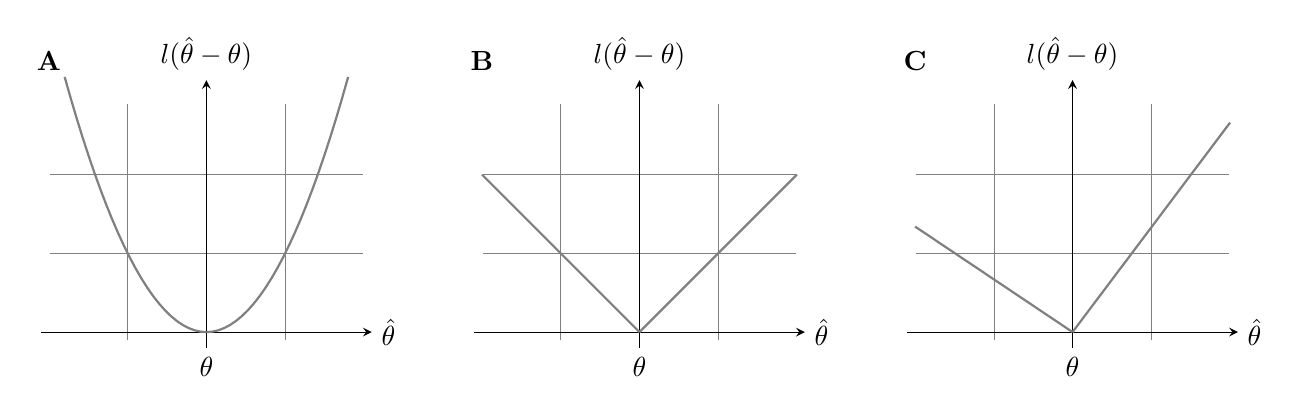
\begin{tikzpicture}%[domain=-1.8:1.8]
\draw[very thin,color=gray] (-1.99,-0.1) grid (1.99,2.9);
\draw[-stealth] (-2.1,0) -- (2.1,0) node[right] {$\hat{\theta}$};
\draw[-stealth] (0,-0.2) node[below] {$\theta$} -- (0,3.2) node[above] {$l(\hat{\theta}-\theta)$};
\draw[color=gray,thick,domain=0:1.8]  plot ({\x},{ \x^2});
\draw[color=gray,thick,domain=-1.8:0] plot ({\x},{-\x^2});
\draw (-2,3.2) node[above] {\textbf{A}};
%
\begin{scope}[xshift=5.5cm]
\draw[very thin,color=gray] (-1.99,-0.1) grid (1.99,2.9);
\draw[-stealth] (-2.1,0) -- (2.1,0) node[right] {$\hat{\theta}$};
\draw[-stealth] (0,-0.2) node[below] {$\theta$} -- (0,3.2) node[above] {$l(\hat{\theta}-\theta)$};
\draw[color=gray,thick,domain=0:2]  plot ({\x},{ \x});
\draw[color=gray,thick,domain=-2:0] plot ({\x},{-\x});
\draw (-2,3.2) node[above] {\textbf{B}};
\end{scope}
%
\begin{scope}[xshift=11cm]
\draw[very thin,color=gray] (-1.99,-0.1) grid (1.99,2.9);
\draw[-stealth] (-2.1,0) -- (2.1,0) node[right] {$\hat{\theta}$};
\draw[-stealth] (0,-0.2) node[below] {$\theta$} -- (0,3.2) node[above] {$l(\hat{\theta}-\theta)$};
\draw[color=gray,thick,domain=0:2]  plot ({\x},{ 1.33*\x});
\draw[color=gray,thick,domain=-2:0] plot ({\x},{-0.67*\x});
\draw (-2,3.2) node[above] {\textbf{C}};
\end{scope}
\end{tikzpicture}
\caption[The quadratic, absolute, and check loss functions.]%
{The quadratic (left), absolute (center), and check (right) loss functions.}
\label{fig:loss}
\end{figure}


The \emph{indicator loss function}
\begin{align*}
l(\hat{\theta}, \theta) = \begin{cases} 0 & |\hat{\theta}-\theta| \le \epsilon \\ 1 & \text{else}\end{cases}\,,
\end{align*}
for $\epsilon \to 0$, leads to the maximum of the posterior,
often abbreviated as MAP (maximum a posteriori) estimator
(see, e.g., \cite{2000:bernardosmith}, \S 5.1.5, p.~257, or \cite{2007:robert}, \S 4.1.2, p.~166).
For a $\be(\nn\yn, \nn(1-\yn))$, the mode is
\begin{align*}
\modus p(\theta\mid\nn, \yn) &= \frac{\nn\yn - 1}{\nn - 2} = \frac{\nz\yz - 1 + s}{\nz - 2 + n}\,,
\end{align*}
and thus is a weighted average of the prior mode $\frac{\nz\yz - 1}{\nz -2}$ $(\nz > 2)$
and the sample proportion $s/n$, with weights $\nz - 2$ and $n$, respectively.

Note that asymptotic optimality properties of maximum likelihood estimators (consistency, efficiency)
are usually preserved for these Baysian point estimators \parencite[e.g.,][Note~1.8.4, pp.~48f]{2007:robert}.

In the Bayesian approach, \textbf{interval estimation} is rather simple,
as the posterior distribution delivers a direct measure of probability for arbitrary subsets of the parameter space $\Theta$.
Mostly, so-called \emph{highest posterior density} (HPD) intervals are considered,
where for a given probability level $\gamma$ the shortest interval covering this probability mass is calculated.
For unimodal densities, this is equivalent to finding a threshold $\alpha$ such that
the probability mass for the set of all $\theta$ with $p(\theta\mid\nn, \yn) \ge \alpha$ equals $\gamma$, hence the name.%
\footnote{See, e.g., \textcite[\S 5.1.5, pp.~259f]{2000:bernardosmith}, or \textcite[Def.~5.5.3, p.~260]{2007:robert}.}
For the Beta posterior, a HPD interval for $\theta$ must be determined by numeric optimisation.
For approximately symmetric (around $\frac{1}{2}$) Beta posteriors, a good approximation is the symmetric credibility interval,
delimited by the $\frac{1-\gamma}{2}$- and the $\frac{1+\gamma}{2}$-quantile of the posterior.

The \textbf{testing of hypotheses} concerning the parameter of interest $\theta$ can be done
by comparing posterior probabilities of two (disjunct) subsets of the parameter space.
Like in frequentist Neyman-Pearson testing, these are often denoted by $\Theta_0$ and $\Theta_1$,
but unlike there, in Bayesian testing the hypotheses $H_0: \theta \in \Theta_0$ and $H_1: \theta \in \Theta_1$ play a symmetric role.
Therefore, it is also possible to express evidence \emph{in favour of} $H_0$,
whereas frequentist tests are constructed such that they can express conclusive evidence only when $H_0$ is rejected.%
\footnote{In Neyman-Pearson testing, only the probability
for the \emph{error of the first kind}, denoted by $\alpha$, of rejecting $H_0$ although it is true, is set to a low predefined level,
whereas the probability for the \emph{error of the second kind}, denoted by $\beta$, of accepting $H_0$ although it is false, may be very large.
$1-\beta$, the probability of correctly rejecting $H_0$, is also known as the \emph{power} of a test.}
However, \emph{point hypotheses}, where one of $\Theta_0$ or $\Theta_1$
consists of a single element of the parameter space only (usually, $\Theta_0 = \{\theta_0\}$),%
\footnote{Such a testing problem is often called \emph{two-sided} in Neyman-Pearson testing.}
require a special treatment if the prior on $\Theta$ is absolutely continuous,
as is the case for the priors \eqref{eq:canonicalprior} considered here,
because then, $\p(\theta \in \Theta_0) = 0$ for any $\theta_0$.
Such an inference task can be considered in terms of a problem of \emph{model selection},
where $\theta = \theta_0$ vs.\ $\theta \neq \theta_0$ decides between two different statistical models,
to each of which a prior probability is assigned \parencite[e.g.,][\S 5.2.4]{2007:robert}.
An overview on Bayesian testing, including a detailed comparison with classical testing procedures,
is given in \textcite[\S 5.2--5.4]{2007:robert}.

Especially in model selection problems, evidence against, or in favor of, a hypothesis
is often not expressed in posterior probability for hypotheses, but by means of the so-called \emph{Bayes factor},
arising when considering odds instead of probability:%
\footnote{See, e.g., \textcite[\S 5.2.2, Def.~5.2.5, p.~227]{2007:robert}, or \textcite[p.~776]{1995:kass-raftery}.}
\begin{align*}
\frac{p(H_1\mid\vec{x})}{p(H_0\mid\vec{x})} &= \frac{f(\vec{x}\mid H_1)}{f(\vec{x}\mid H_0)} \cdot \frac{p(H_1)}{p(H_0)}
\end{align*}
Here, the factor
\begin{align*}
B_{10} &:= \frac{f(\vec{x}\mid H_1)}{f(\vec{x}\mid H_0)}\,,
\end{align*}
translating prior to posterior odds, is the Bayes factor for comparing $H_1$ to $H_0$.%
\footnote{Usually, more than two hypotheses are considered in model selection,
by comparing competing models $H_1, H_2, \ldots$ to a null model $H_0$
with help of Bayes factors $B_{10}, B_{20}, \ldots$.}

Improper priors are problematic in Bayesian testing \parencite[\S 5.2.5]{2007:robert}
and should be avoided for parameters the test decides upon \parencite[p.~782]{1995:kass-raftery}.%
\footnote{\Textcite[\S 5.5.4 (j)]{1991:walley} gives an instructing example for the problems
that arise in testing with so-called non-informative priors.}
We see this as a strong argument against the use of improper priors.
An example where improper priors seem inadequate also for parameter estimation
will be given in Section~\ref{sec:alpha-factor-prior};
comments on improper priors from the viewpoint of generalised Bayesian inference
are given in Section~\ref{sec:gbicp-properties-criteria},
item \ref{enum:noninformative}, and in Section~\ref{sec:idm-and-near-ignorance}.

%Sections~\ref{sec:motivation:near-ignorance}, .
\iffalse
\cite[p.~235f]{2007:robert}
\begin{quote}
The difficulties encountered with noninformative priors in testing
also point out that a testing problem cannot be treated in a coherent way if no prior information is available,
that is, that the information brought by the observations alone is usually not enough
to infer about the truth of a hypothesis in categorical fashion (\emph{yes}/\emph{no}).
This obviously reinforces the the motivation for a Bayesian treatment of such testing problems,
since it is the only coherent approach taking advantage of the residual information.
\end{quote}
\fi

%Can express evidence \emph{in favour of} point-null hypothesis (Kass \& Raftery).
%The problem with point-null hypotheses (Robert)???
%Model selection mostly and Testing closely related.

%equivalence of posterior probability for $H_0$ (or $H_1$) and Bayes factor \cite[p.~227]{2007:robert}
%High values of $P(H_1\mid\x) / P(H_0\mid\x)$ then indicate high plausibility of $H_1$ as compared to $H_0$.
%Article on Bayes factors as entity of its own: Kass \& Raftery 1995: Bayes factor and model uncertainty, JASA 90, 773--795


The \textbf{posterior predictive} distribution, giving the probability for $s^*$ successes in $n^*$ future trials
after having seen $s$ successes in $n$ trials, is
\begin{align*}
f(s^* \mid \nn, \yn) &= {n^* \choose s^*} \frac{\B\big(s^* + \nn \yn, n^* - s^* + \nn (1 - \yn)\big)}{\B\big(\nn\yn, \nn (1 - \yn)\big)}\,,
\end{align*}
known as the \emph{Beta-Binomial distribution}.%
\footnote{Section~\ref{sec:isipta11} discusses imprecise Bayesian inference in the Beta-Binomial model,
studying the probability of the next observation to be a success in dependence on the number of successes $s$ in $n$ past observations.}


\subsubsection{The Normal-Normal Model}
\label{sec:norm-norm}

%***add comment on general case $\vartheta=(\mu,\sigma^2)$***\\
The normal density \eqref{eq:normaldens}, here with the variance $\sigma^2$ known to be equal to $\sigma^2_0$,
also adheres to the exponential family form:
\begin{align*}
f(\x \mid \mu, \sigma_0^2)
 &\propto \exp\Big\{ \frac{\mu}{\sigma_0^2} \sum_{i=1}^n x_i - \frac{n\mu^2}{2\sigma_0^2} \Big\}.
\end{align*}
So we have here $\psi = \frac{\mu}{\sigma_0^2}$, $\mbf{b}(\psi) = \frac{\mu^2}{2\sigma_0^2}$, and $\tau^*(x_i) = x_i$.
From these ingredients, a conjugate prior can be constructed with \eqref{eq:canonicalprior}, leading to
\begin{align*}
p\Big(\frac{\mu}{\sigma_0^2} \mid \nz, \yz\Big) \dd\frac{\mu}{\sigma_0^2}
 &\propto \exp\Big\{ \nz \Big( \langle \yz, \frac{\mu}{\sigma_0^2} \rangle - \frac{\mu^2}{2\sigma_0^2} \Big) \Big\} \dd\frac{\mu}{\sigma_0^2}\,.
\end{align*}
This prior, transformed to the parameter of interest $\mu$ and with the square completed,
\begin{align*}
p(\mu \mid \nz, \yz) \dd\mu
 &\propto \frac{1}{\sigma_0^2} \exp\Big\{ -\frac{\nz}{2\sigma_0^2} (\mu - \yz)^2 \Big\} \dd\mu\,,
\end{align*}
is a normal distribution with mean $\yz$ and variance $\frac{\sigma_0^2}{\nz}$,
i.e.\ $\mu \sim \norm(\yz, \frac{\sigma_0^2}{\nz})$.%
\footnote{The conjugate prior if both $\mu$ and $\sigma^2$ are unknown
is the so-called normal-inverse gamma distribution,
a combination of the normal distribution above and the inverse gamma distribution
\parencite[see, e.g.,][pp.~119, 431]{2000:bernardosmith}.
This prior is a special case of the priors for Bayesian regression discussed in Section~\ref{sec:festschrift},
where $\X = (1, \ldots, 1)^\tra$ and $\bbeta = \mu$.
When instead of the variance $\sigma^2$ the precision $\kappa = 1/\sigma^2$ is considered,
this prior can be written as a normal-gamma prior
\parencite[see, e.g.,][pp.~136, 434]{2000:bernardosmith}.}

With \eqref{eq:canonicalupdate}, the parameters for the posterior distribution are
\begin{align}
\yn &= \E[\mu\mid\nn, \yn] = \frac{\nz}{\nz + n} \cdot \yz + \frac{n}{\nz + n} \cdot \bar{x} \label{eq:normalposte}\\
\frac{\sigma_0^2}{\nn} &= \V(\mu\mid\nn, \yn) = \frac{\sigma_0^2}{\nz + n}\,. \label{eq:normalpostvar}
\end{align}
The posterior expectation of $\mu$ thus is a weighted average of the prior expectation $\yz$ and the sample mean $\bar{x}$,
with weights $\nz$ and $n$, respectively.
The effect of the update step on variance is that it decreases by the factor $\nz/(\nz+n)$.

Here, all of the three standard choices of loss functions mentioned for the Beta-Binomial model
lead to the same \textbf{point estimator} $\hat{\mu} = \yn$,
as in normal distributions mean, median, and mode coincide.

As \textbf{interval estimation}, the HPD interval can be calculated, due to symmetry of the normal posterior,
as $[z\un_\frac{1-\gamma}{2}, z\un_\frac{1+\gamma}{2}]$, where, e.g.,
$z\un_\frac{1-\gamma}{2}$ is the $\frac{1-\gamma}{2}$-quantile of the normal distribution with mean $\yn$ and variance $\frac{\sigma_0^2}{\nn}$.

The \textbf{testing of hypotheses} about $\mu$ works again by comparing posterior probabilities of two disjunct subsets of the parameter space.
Note that the frequentist analogue to such a test is the (one-sided) one-sample Z-test (or Gaussian test).

The \textbf{posterior predictive} distribution for $n^*$ future observations denoted by $\x^*$ is again a normal distribution,
$\x^*\mid \nn,\yn \sim \norm\big(\yn, \frac{\sigma_0^2}{\nn}(\nn + n^*)\big)$,
centered at the posterior mean \eqref{eq:normalposte},
and with variance increasing with the posterior variance \eqref{eq:normalpostvar}
and the number of observations to be predicted.


\subsubsection{The Dirichlet-Multinomial Model}
\label{sec:diri-multi}

The construction of the canonical conjugate prior by Eq.~\eqref{eq:canonicalprior}
for the Multinomial model $\mult(\btheta)$ with $k>2$ is more complex than for the case $k=2$
as covered in Section~\ref{sec:beta-binom}.
It is a well-known result that this construction leads to the commonly used Dirichlet prior;
however, in the literature the construction is usually not derived in detail.%
\footnote{E.g., \textcite[Table~1]{2005:quaeghebeurcooman} tabulate, without proof,
priors constructed for a number of sample models.
Note that the first version of the paper contains a sign error in the $\mbf{b}(\bpsi)$ column
for both the Binomial (Bernoulli) and the Multinomial (multivariate Bernoulli) sampling model.}
We will cover the construction of $p(\bpsi\mid\nz, \yz)$,
and also the transformation to $p(\btheta\mid\nz, \yz)$,
in more detail here.

We will use the formulation of $\mult(\btheta)$ as the multivariate Bernoulli distribution
like in Example~\ref{ex:multinomdist}. %Section~\ref{sec:multinomdist}.
The distribution of a single multivariate Bernoulli observation is equivalent to a Multinomial distribution with sample size $1$,
and i.i.d.\ repetitions of a multivariate Bernoulli distribution lead to the Multinomial distribution.
Since i.i.d.\ repetitions do not interfere with conjugacy
(as mentioned in Footnote~\ref{foot:dataisplural}, page~\pageref{foot:dataisplural}.),
we may construct the canonical conjugate prior by considering a single multivariate Bernoulli observation.

To do without side conditions like $\sum_{j=1}^k \theta_j = 1$ as needed in Example~\ref{ex:multinomdist}, %Section~\ref{sec:multinomdist},
we will define here as a single multivariate Bernoulli observation distinguishing $k+1$ categories $j = 0,1,\ldots,k$
(instead of $k$ categories $j = 1,\ldots,k$ as in Example~\ref{ex:multinomdist}) %Section~\ref{sec:multinomdist})
a vector $\x$ with $k$ components indexed $1,\ldots,k$
such that
\begin{align*}
\x \in \{0,1\}^k \cap \big\{ \x: \sum_{j=1}^k x_j \in \{0,1\}  \big\}\,,
\end{align*}
and $x_0 := 1 - \sum_{j=1} x_j$.

The parameter vector is treated in the same way, i.e.,
we consider now $\btheta$ with $k$ components $\theta_j, j=1,\ldots,k$ such that
\begin{align*}
\btheta \in (0,1)^k \cap \{\btheta: 0 < \sum_{j=1}^k \theta_j < 1\}\,,
\end{align*}
and thus $\theta_0 := 1-\sum_{j=1}^k \theta_j$.

Formulating the density \eqref{eq:multinomdens} accordingly, and rewriting it towards~\eqref{eq:expofam-sampledens},
we get
\begin{align*}
p(\x\mid\btheta)&= \Bigg( \prod_{j=1}^k \theta_j^{x_j}\Bigg) \bigg( 1 - \sum_{j=1}^k \theta_j\bigg)^{1-\sum_{j=1}^k x_j}%\\
                 = \theta_0 \prod_{j=1}^k \left(\frac{\theta_j}{\theta_0}\right)^{x_j} \\
                &= \exp\Bigg\{ \sum_{j=1}^k x_j \ln\bigg(\frac{\theta_j}{\theta_0}\bigg) - \big(-\ln(\theta_0)\big) \Bigg\}\,.
\end{align*}
With $\bpsi$ and $\mbf{b}(\bpsi)$ derived from the sample model as
\begin{align*}
\psi_j &= \ln\left(\frac{\theta_j}{\theta_0}\right),\, j=1,\ldots,k & \text{and}& &
\mbf{b}(\bpsi) &= -\ln(\theta_0),\,% \theta_0 = 1 - \sum_{j=1}^k \theta_j\,,
\end{align*}
the conjugate prior is at first constructed as a density over $\bpsi$,
dropping the upper index ${}\uz$ in $\nz$ and the vectorial $\byz$ for ease of notation:
\begin{align*}
p(\bpsi\mid n,\vec{y})\, \dd\bpsi
 &\propto \exp\Bigg\{n\, \Bigg[ \sum_{j=1}^k y_j \ln\bigg(\frac{\theta_j}{\theta_0}\bigg) - \big(-\ln(\theta_0)\big) \Bigg] \Bigg\} \,\dd\bpsi\,,.
\end{align*}
Written as a density over $\btheta$, we have
\begin{align*}
p(\btheta\mid n,\vec{y})\, \dd\btheta
 &\propto \exp\Bigg\{n\, \Bigg[ \sum_{j=1}^k y_j \ln\bigg(\frac{\theta_j}{\theta_0}\bigg) - \big(-\ln(\theta_0)\big) \Bigg] \Bigg\}
  \cdot \left| \det\left(\frac{\dd\bpsi}{\dd\btheta}\right) \right|\, \dd\btheta\,,
\end{align*}
with the elements of the Jacobian matrix $\dfrac{\dd\bpsi}{\dd\btheta}$ being
\begin{align*}
\frac{\dd\psi_i}{\dd\theta_i} &= \frac{1}{d\theta_i} \ln\left(\frac{\theta_i}{1 - \sum_{j=1}^k \theta_j}\right)
                               = \frac{1-\sum_{j=1}^k \theta_j}{\theta_i}
                                 \cdot \frac{1 - \sum_{j=1}^k \theta_j + \theta_i}{(1 - \sum_{j=1}^k \theta_j)^2}
                               = \frac{\theta_0 + \theta_i}{\theta_0 \theta_i}\\
\frac{\dd\psi_h}{\dd\theta_i} &= \frac{1}{d\theta_i} \ln\left(\frac{\theta_h}{1 - \sum_{j=1}^k \theta_j}\right)
                               = \frac{1-\sum_{j=1}^k \theta_j}{\theta_h} \cdot \frac{\theta_h}{(1 - \sum_{j=1}^k \theta_j)^2}
                               = \frac{1}{\theta_0}\,, \quad h \neq i
\end{align*}
\allowdisplaybreaks
Thus,
\begin{align*}
\det\left(\frac{\dd\bpsi}{\dd\btheta}\right)
&= \det \begin{pmatrix}\frac{\theta_0 + \theta_1}{\theta_0 \theta_1} & \frac{1}{\theta_0} & \hdots & \frac{1}{\theta_0} \\
                       \frac{1}{\theta_0} & \frac{\theta_0 + \theta_2}{\theta_0 \theta_2} & \ddots & \vdots \\
                       \vdots & \ddots & \ddots & \frac{1}{\theta_0} \\[1ex]
                       \frac{1}{\theta_0} & \hdots & \frac{1}{\theta_0} & \frac{\theta_0 + \theta_k}{\theta_0 \theta_k}
        \end{pmatrix} \\
&= \left(\frac{1}{\theta_0}\right)^k\, \det
        \begin{pmatrix}\frac{\theta_0}{\theta_1} + 1 & 1 & \hdots & 1 \\
                       1 & \frac{\theta_0 }{\theta_2} + 1 & \ddots & \vdots \\
                       \vdots & \ddots & \ddots & 1 \\[1ex]
                       1 & \hdots & 1 & \frac{\theta_0}{\theta_k} + 1
        \end{pmatrix} \\
&\stackrel{*}{=} \left(\frac{1}{\theta_0}\right)^k \prod_{j=1}^k \frac{\theta_0}{\theta_j}
                 \cdot \Bigg( 1 + \begin{pmatrix}1 & \hdots & 1\end{pmatrix}
                                  \begin{pmatrix}\frac{\theta_1}{\theta_0} &  & 0 \\
                                                  & \ddots & \\
                                                 0 & & \frac{\theta_k}{\theta_0}\end{pmatrix}
                                  \begin{pmatrix}1 \\ \vdots\\ 1\end{pmatrix}\Bigg)\\
&= \prod_{j=1}^k \frac{1}{\theta_j} \cdot \Bigg( 1 + \sum_{i=1}^k \frac{\theta_i}{\theta_0} \Bigg)
 = \Bigg( \prod_{j=1}^k \frac{1}{\theta_j}\Bigg) \frac{ \theta_0 + \sum_{i=1}^k \theta_i}{\theta_0}\\
&= \Bigg( \prod_{j=1}^k \frac{1}{\theta_j}\Bigg) \frac{1}{\theta_0}
 = \prod_{j=0}^k \frac{1}{\theta_j}\,,
\end{align*}
where equality ${}^*$ holds by the theorem 
%in Rao, Toutenburg, Shalabh, and Heumann, \emph{Linear models and generalizations}, Springer, Berlin 2008: %bibtex at end of document
%stating that
\begin{align*}
\det (\mbf{A} + \vec{a}\, \vec{a}^\tra) &= \det(\mbf{A}) (1+\vec{a}^\tra \mbf{A}^{-1} \vec{a}) %& \text{if}& & \det(\mbf{A}) &\neq 0
\end{align*}
for all column vectors $\vec{a}$ and appropriately sized, invertible matrices $\mbf{A}$ 
\parencite[Theorem A 16 (x), Appendix A3, p.~494]{MR2370506}.

With $\det\left(\frac{\dd\bpsi}{\dd\btheta}\right) = \prod_{j=0}^k \frac{1}{\theta_j}$, we get
\begin{align*}
\allowdisplaybreaks
p(\btheta\mid n,\vec{y})
 &\propto \exp\Bigg\{n\, \Bigg[ \sum_{j=1}^k y_j \ln\bigg(\frac{\theta_j}{\theta_0}\bigg) - \big(-\ln(\theta_0)\big) \Bigg] \Bigg\}
  \cdot \bigg| \prod_{j=0}^k \frac{1}{\theta_j} \bigg| \\
 &=       \exp\Bigg\{n\, \Bigg[ \sum_{j=1}^k y_j \Big(\ln(\theta_j)-\ln(\theta_0)\Big) + \ln(\theta_0) \Bigg]
                         - \sum_{j=0}^k \ln(\theta_j) \Bigg\} \\
 &=       \exp\Bigg\{n\, \Bigg[ \sum_{j=1}^k y_j \ln(\theta_j) + \ln(\theta_0) \bigg(\underbrace{1 - \sum_{j=1}^k  y_j}_{=: y_0}\bigg) \Bigg]
                         - \sum_{j=0}^k \ln(\theta_j) \Bigg\} \\
 &=       \exp\Bigg\{n\, \Bigg[ \sum_{j=0}^k y_j \ln(\theta_j) \Bigg] - \sum_{j=0}^k \ln(\theta_j) \Bigg\} \\
 &=       \exp\Bigg\{\sum_{j=0}^k (n\,y_j -1 ) \ln(\theta_j) \Bigg\}
  =       \exp\Bigg\{\sum_{j=0}^k \ln\left(\theta_j^{n\,y_j -1}\right) \Bigg\}\\
 &= \prod_{j=0}^k \theta_j^{n\,y_j - 1}\,,
\end{align*}
which is the core of a Dirichlet density over $\btheta$.
Therefore, the Dirichlet distribution is the canonically constructed conjugate prior to the multivariate Bernoulli.
Due to the considerations from the beginning of this section,
we see that the Dirichlet distribution is the canonically constructed conjugate prior
also to the Multinomial sample model with arbitrary sample sizes.

The Dirichlet distribution can be seen as a direct generalisation of the Beta distribution,
and we will speak of the \emph{Dirichlet-Multinomial model}
as the analogue to the Beta-Binomial model from Section~\ref{sec:beta-binom}.

Returning to the notation from Example~\ref{ex:multinomdist}, %Section~\ref{sec:multinomdist},
where $k$ categories $j=1,\ldots,k$ are considered, 
we have thus
\begin{align}
\label{eq:dirichlet-prior}
p(\btheta\mid\nz,\byz) \propto \prod_{j=1}^k \theta_j^{\nz\yz_j-1}
\end{align}
as the prior.
The vectorial $\byz$ is an element of the interior of the $k-1$-dimensional unit simplex $\Delta$,
thus $\forall j \ \yz_j \in (0,1)$, $\sum_{j=1}^k \yz_j = 1$, in short $\byz \in \text{int}(\Delta)$.
Here, the main posterior parameter is calculated as
\begin{align*}
\yn_j &= \frac{\nz}{\nz+n} \yz_j + \frac{n}{\nz+n} \cdot \frac{n_j}{n}\,,\quad j = 1,\ldots, k,
\end{align*}
and is thus again a weighted average of the main prior parameter
(which can be interpreted as prior guess for $\btheta$, as $\E[\btheta\mid\nz,\byz] = \byz$)
and the fractions of observations in each category,
with weights $\nz$ and $n$, respectively.
$\nz$ again governs the concentration of probability mass around $\yz$,
with larger values of $\nz$ leading to higher concentrations.

With these tangible intuitions for $\nz$ and $\byz$,
we will denote the Dirichlet prior directly in terms of the canonical parameters, i.e.\ by
%\begin{align*}
$\btheta \sim \dir(\nz,\byz)$.
%\end{align*}
The canonical parameters relate to the commonly used parameter, often denoted by $\bs{\alpha} = (\alpha_1, \ldots, \alpha_k)$, 
not to be confused with $\vec{\alpha}$ as discussed in Section~\ref{sec:alpha-factor-model}, via%
\begin{align*}
\yz_j &= \frac{\alpha_j}{\sum_{l=1}^k \alpha_l} &
\nz   &= \sum_{l=1}^k \alpha_l \,.
\end{align*}

We will now present a problem in reliability analysis for which the most common model
relies on the Dirichlet-Multinomial model.
The issues encountered in this application that is based on
\textcite{Troffaes2013a} will motivate the use of sets of distributions as prior models,
illustrating the advantages in uncertainty modelling that can be gained from using imprecise probability models.%
\footnote{Basic aspects of the theory of imprecise probability,
and further motivations for using it, will be given in Chapter~\ref{cha:gbi}.}
The models discussed there will then be integrated into a general framework
of inference using sets of canonical conjugate priors in Section~\ref{sec:generalmodel}.

\newpage

\section{Dirichlet-Multinomial Model for Common-Cause Failure}
\label{sec:commoncause}

In reliability analysis of systems with redundant components,
\emph{common-cause failure} refers to simultaneous failure of several redundant components due to a common or shared root cause,
like extreme environmental conditions (e.g., fire, flood, or earthquake) \parencite[p.~325]{1994:hoyland}.
It has been recognized as the dominant factor to the unreliability of redundant systems,
and its modeling has become an important part of reliability analysis
following the Reactor Safety Study \parencite{1975:reactor:safety:study},
which was prepared in the wake of the Three Mile Island accident,
where a partial core meltdown in a nuclear power plant took place \parencite[e.g.,][]{2005:walker}.

\subsection{An Example for the Need to Model Common-Cause Failure}
\label{sec:commoncause-motivation}

For a nuclear power plant, a common-cause failure analysis can relate to, e.g.,
the diesel generators that, if in an emergency the off-site power supply is cut off,
provide the electricity to power the emergency core cooling systems.
Emergency core cooling systems are needed to transfer away residual heat emitted from the core after shutdown,
in case the normal heat removal process%
\footnote{Heat from the core is transferred to steam generators,
producing steam that drives turbines linked to generators producing electricity.
Usually, the depressurized steam exiting the turbines
is then condensated to water, which is fed back into the steam generators.}
is not available.
When residual heat is not removed, it can overheat the core,
which could lead to a (partial) core meltdown,
and subsequently to a possibly catastrophic release of radioactive material.%
\footnote{The residual heat that is present in the core of a nuclear power plant
after shutdown of the nuclear chain reaction is called \emph{decay heat}.
It results from secondary decay processes,
i.e.\ from the decay of fission products produced during normal operation of the power plant.
Although comprising only a small fraction of the energy output during normal operation
(where the energy stems from the primary fission process \parencite[Module~4, p.~33]{united1993doe}),
depending on the design of the reactor,
the decay heat may be enough to damage the core of a reactor significantly
\parencite[pp.~VIII-9 and VIII-25f]{1975:reactor:safety:study}.}

Due to their critical role for the functioning of emergency cooling systems,
and thus for the safety systems of nuclear power plants in general \parencite[pp.~1, 4]{csni86-115},
there are usually several diesel generators installed in a nuclear power plant,
each of which can supply enough energy to power the cooling systems on its own.
The number of diesel generators installed is typically in the range of two to four per reactor
%**EPRI NP-2433 ??***.
(see, e.g., \textcite{csni86-115}, pp.~121, 145).
If the nuclear power plant has several reactors, diesel generators may be shared between reactors \parencite[p.~7]{2004:iaea::emergencypower}.
%i.e., there are four redundant components, of which one is needed for service.
%with a redundancy in the order of four or 
The Fukushima Daiichi nuclear disaster is a recent example of an accident
involving common cause failure of diesel generators.
In this case, all 12 available diesel generators at reactors 1 to 6 
ceased to function due to a tsunami wave flooding the rooms where they were installed \parencite[p.~31]{2011:iaea::report}.
The tsunami wave had been caused by the T\={o}hoku earthquake \parencite[e.g.,][]{2012:ritsema},
which had promted the reactors to shutdown automatically, and in doing so,
switching to the diesel generators for power supply.%
\footnote{All six off-site power lines were cut off, also due to the earthquake \parencite[p.~31]{2011:iaea::report}.}

The arguably most widely used model for common-cause failure is the so-called \emph{Basic Parameter Model}.
The \emph{alpha-factor} parametrisation of this model uses a multinomial distribution
as its aleatory model for observed failures \parencite{1988:mosleh::common:cause}. 
As seen in Section~\ref{sec:diri-multi}, the conjugate prior to the multinomial model is the Dirichlet distribution.
In the standard Bayesian approach, the analyst specifies the parameters $(\nz, \byz)$ of a precise Dirichlet distribution
to model epistemic uncertainty in the alpha-factors, which are the parameters of the multinomial sample model.
%This Dirichlet prior is then updated with observed data to obtain a precise posterior distribution, also Dirichlet.

We will first describe the Basic Parameter Model in its standard form,
and subsequently present its reparametrisation in terms of alpha-factors.


\subsection{The Basic Parameter Model}
\label{sec:basic-param-model}

Consider a system that consists of $k$ components.
Throughout, we make the following standard assumptions:
\begin{inparaenum}[(i)]
\item repair is immediate, and
\item failures follow a Poisson process.
\end{inparaenum}

For simplicity, we assume that all $k$ components are exchangeable,
in the sense that they have identical failure rates.
More precisely,
we assume that all events involving \emph{exactly} $j$ components failing
have the same failure rate, which we denote by $q_j$.
This model is called the \emph{basic parameter model},
and we write $\vec{q}$ for $(q_1,\dots,q_k)$.

For example, if we have three components, A, B, and C,
then the rate at which we see only A failing
is equal to the rate at which we see only B failing,
and is also equal to the rate at which we see only C failing;
this failure rate is $q_1$.
Moreover, the rate at which we observe only A and B jointly failing
is equal to the rate at which we observe only B and C jointly failing,
and also equal to the rate at which we observe only A and C jointly failing;
this failure rate is $q_2$.
The rate at which we see all three components jointly failing is $q_3$.

In case of $k$ identical components without common-cause failure modes,
thus each failing independently at rate $\lambda$, we would have%
\footnote{This is due to our Poisson assumption, and the assumption of immediate repair:
independent Poisson processes never generate events simultaneously when we observe failure times precisely.}
\begin{equation*}
  q_1=\lambda\qquad \text{ and }\qquad q_j=0\text{ for }j\ge 2.
\end{equation*}
The fact that we allow arbitrary values for the $q_j$ reflects
the lack of independence, and whence, our modelling of common-cause failures.
At this point, it is worth noting that we do not actually write down a statistical model
for all possible common-cause failure modes---we could do so if this information was available,
and in fact, this could render the basic parameter model obsolete,
and allow for more detailed inferences.
In essence, the basic parameter model allows us to statistically model
lack of independence between component failures,
without further detail as to where dependencies arise from:
all failure modes are lumped together, so to speak.

It is useful to note that it is possible, and sometimes necessary,
to relax the exchangeability assumption
to accommodate specific asymmetric cases.
For example, when components are in different state of health,
single failures would clearly not have identical failure rates.
Because the formulas become a lot more complicated,
we stick to the exchangeable case here.%
\footnote{A discussion of the asymmetric case, i.e., without the assumption of exchangeability of components,
can be found in \textcite{2013:troffaes-blake}.}

Clearly, to answer typical reliability questions, such as for instance
``what is the probability that two or more components fail in the next month?'',
we need $\vec{q}$.
In practice, the following three issues commonly arise.
First, $\vec{q}$ is rarely measured directly,
as failure data is often collected only per component.
Secondly, when direct data about joint failures is available,
typically, this data is sparse,
because events involving more than two components failing simultaneously are usually quite rare.
Thirdly, there are usually two distinct sources of failure data,
one usually very large data set related to failure per component,
and one usually much smaller data set related to joint failures.
For these reasons,
it is sensible to reparametrise the model in terms
of parameters that can be more easily estimated, as follows.


\subsection{The Alpha-Factor Model}
\label{sec:alpha-factor-model}

The alpha-factor parametrisation of the basic parameter model
\parencite{1988:mosleh::common:cause} starts out with
considering the total failure rate of a component $q_t$,
which could involve failure of any number of components,
that is, this is the rate obtained by looking at just one component,
ignoring everything else.
Clearly,
\begin{equation}\label{eq:qt:in:terms:of:qj}
  q_t=\sum_{j=1}^k\binom{k-1}{j-1}q_j.
\end{equation}
For example, again consider a three component system, A, B, and C.
The rate at which A fails is then
the rate at which only A fails ($q_1$),
plus the rate at which A and B, or A and C fail ($2q_2$),
plus the rate at which all three components fail ($q_3$).

Next, the alpha-factor model introduces
$\alpha_j$---the so-called alpha-factor---which
denotes the probability of \emph{exactly} $j$ of the $k$ components
failing given that failure occurs;
in terms of relative frequency,
$\alpha_j$ is the fraction of failures
that involve \emph{exactly} $j$ failed components.
We write $\vec{\alpha}$ for $(\alpha_1,\dots,\alpha_k)$.
Clearly,
\begin{equation}\label{eq:alphaj:in:terms:of:qj}
  \alpha_j=\frac{\binom{k}{j}q_j}{\sum_{\ell=1}^k\binom{k}{\ell}q_\ell}.
\end{equation}
For example, again consider A, B, and C.
Then the rate at which exactly one component fails is $3q_1$
(as we have three single components, each of which failing with rate $q_1$),
the rate at which exactly two components fail is $3q_2$
(as we have three combinations of two components,
each combination failing with rate $q_2$),
and the rate at which all components fail is $q_3$.
Translating these rates into fractions,
we arrive precisely at Eq.~\eqref{eq:alphaj:in:terms:of:qj}.

It can be shown that \parencite[e.g.,][p.~C-10f]{1988:mosleh::common:cause} %:\footnote{Hint: consider $\sum_{j=1}^k j\alpha_j$.}
\begin{equation}\label{eq:qj:in:terms:of:qt}
  q_j=\frac{1}{\binom{k-1}{j-1}}\frac{j\alpha_j}{\sum_{\ell=1}^k \ell\alpha_\ell}\,q_t\,.
\end{equation}
Eqs.~\eqref{eq:qt:in:terms:of:qj}, \eqref{eq:alphaj:in:terms:of:qj},
and~\eqref{eq:qj:in:terms:of:qt}
establish a one-to-one link between the basic parameter model (with parameters $\vec{q}$)
and the alpha-factor model (with parameters $q_t$, $\vec{\alpha}$).
The benefit of the alpha-factor model over the basic parameter model
lies in its distinction between the total failure rate of a component $q_t$,
for which there is generally a lot of information,
and common-cause failures modelled by $\vec{\alpha}$,
for which there is generally very little information.

Next, we will show how we can use the Dirichlet-Multinomial model
from Section~\ref{sec:diri-multi} to estimate the alpha factors $\vec{\alpha}$.
Estimating the marginal failure rate $q_t$ is possible in the framework from Section~\ref{sec:regularconjugates} as well,
when failures are assumed to follow a Poisson process.
Then, the Gamma prior usually specified for the intensity parameter is of the form \eqref{eq:canonicalprior}.
We will not cover such a \emph{Gamma-Poisson model} here further,
but details for this model can be found in \textcite{Troffaes2013a}.
There, also the combination of the Dirichlet-Multinomial model for $\vec{\alpha}$
and the Gamma-Poisson model for $q_t$ to make inferences on $\vec{q}$ is discussed.


\subsection{Dirichlet Prior for Alpha-Factors}
\label{sec:alpha-factor-prior}

Suppose that we have observed a sequence of $n$ failure events,
where we have counted the number of components involved with each failure event,
say $n_j$ of the $n$ observed failure events involved \emph{exactly} $j$ failed components.
As in Example~\ref{ex:multinomdist}, %Section~\ref{sec:multinomdist},
we write $\vec{n}$ for $(n_1,\dots,n_k)$.
With the alpha-factors taking the role of the parameter $\btheta$ in \eqref{eq:multinomdens},
the multinomial sample model for $\vec{n}$ has the form
\begin{equation*}
%  \label{eq:multinomial:likelihood}
f(\vec{n}\mid\vec{\alpha}) \propto \prod_{j=1}^k\alpha_j^{n_j}\,.
\end{equation*}

As mentioned already, in this application of multinomial sample model,
the $n_j$ are usually very low for $j\ge 2$,
with zero being quite common for larger $j$.
In such cases, standard techniques such as maximum likelihood for estimating the alpha-factors fail to produce sensible inferences.
For any inference to be reasonably possible, it has been recognized \parencite{1988:mosleh::common:cause}
that we have to rely on epistemic information, that is, information which is not just described by the data.

A standard way to include epistemic information in the model is
through specification of the conjugate Dirichlet prior \eqref{eq:dirichlet-prior} for the alpha-factors \parencite{1988:mosleh::common:cause},
i.e., using the Dirichlet-Multinomial model for inferences about $\vec{\alpha}$:
\begin{equation*}
%\label{eq:dirichlet-prior-alpha}
p(\vec{\alpha}\mid\nz,\byz) \propto \prod_{j=1}^k\alpha_j^{\nz\yz_j-1}
\end{equation*}

To recap, $\nz>0$ and $\byz\in\Delta$, where $\Delta$ is the $(k-1)$-dimensional unit simplex:
\begin{equation*}
\Delta=\left\{
(\yz_1,\dots,\yz_k)\colon \yz_1\ge 0,\dots,\yz_k\ge 0,\,\sum_{j=1}^k \yz_j=1
\right\}
\end{equation*}
%An interpretation for these parameters will be given shortly.
Calculating the posterior density for $\vec{\alpha}$ then results in
\begin{align*}
p(\vec{\alpha}\mid\nz,\byz, \vec{n})
 &= p(\vec{\alpha}\mid\nn,\byn)
 \propto \prod_{j=1}^k\alpha_j^{\nn\yn_j-1} 
 = \prod_{j=1}^k\alpha_j^{\nz\yz_j+n_j-1}\,.
\end{align*}

Of typical interest is for instance the posterior expectation of the probability $\alpha_j$
of observing $j$ of the $k$ components failing due to a common cause given that failure occurs,
\begin{align}
\label{eq:dirichlet:posterior:predictive}
\E[\alpha_j\mid\nz,\byz,\vec{n}]
 &= \int_{\Delta}\alpha_j p(\vec{\alpha}\mid\nz,\byz,\vec{n})\dd\vec{\alpha}\nonumber\\
 &= \frac{\nz\yz_j+n_j}{\nz+n}
  = \frac{\nz}{\nz+n} \yz_j + \frac{n}{\nz+n} \frac{n_j}{n}\,,
\end{align}
where $n=\sum_{j=1}^k n_j$ is the total number of observations.

Eq.~\eqref{eq:dirichlet:posterior:predictive} provides the interpretation for the hyperparameters
$\nz$ and $\byz$ as mentioned in Section~\ref{sec:diri-multi},
discussed here in terms of the alpha-factor model:
\begin{itemize}
\item If $n=0$, then $\E[\alpha_j\mid\nz,\byz,\vec{n}]=\yz_j$,
so $\yz_j$ is the prior expected chance of observing $j$ of the $k$ components failing due to a common cause,
given that failure occurs.
\item $\E[\alpha_j\mid\nz,\byz,\vec{n}]$ is a weighted average of $\yz_j$ and $n_j/n$
(the proportion of $j$-component failures in the $n$ observations), with weights $\nz$ and $n$, respectively.
The parameter $\nz$ thus determines how much data is required for the posterior to start moving away from the prior.
If $n \ll \nz$ then the prior will weigh more;
if $n = \nz$, then prior and data will weigh equally;
and if $n \gg \nz$, then the data will weigh more.
In particular, $\E[\alpha_j\mid\nz,\byz,\vec{n}]=\yz_j$ if $n=0$ (as already mentioned),
and $\E[\alpha_j\mid\nz,\byz,\vec{n}] \to \frac{n_j}{n}$ as $n \to \infty$.
\end{itemize}


\subsection{Usual Handling of Epistemic Information for Alpha-Factors}
\label{sec:epistemic-alpha}

Crucial to reliable inference in the alpha-factor model
is proper modelling of epistemic information about failures,
which is in the above approach expressed through the choice of $(\nz,\byz)$.
By means of an example taken from \textcite{2011:kelly:atwood},
we will demonstrate that posterior inferences rely crucially on this choice of hyperparameters,
particularly when faced with zero counts.

%We focus on two methods for elicitation of these parameters, and the inferences that result from them.

Consider a system with four redundant components ($k=4$).
The probability of $j$ out of $k$ failures, given that failure has happend, was denoted by $\alpha_j$.
We assume that the analyst's prior expectation $\mu_{\text{spec},j}$ for each $\alpha_j$ is:
\begin{align}
  \label{eq:example:muspec}
  \mu_{\text{spec},1} &= 0.950
  &
  \mu_{\text{spec},2} &= 0.030
  &
  \mu_{\text{spec},3} &= 0.015
  &
  \mu_{\text{spec},4} &= 0.005
\end{align}
We have 36 observations, in which 35 showed one component failing,
and 1 showed two components failing:
\begin{align*}
  n_1 &= 35
  &
  n_2 &= 1
  &
  n_3 &= 0
  &
  n_4 &= 0
\end{align*}

\textcite{1996:atwood} studied priors for the binomial model
which maximise entropy (and whence, are `non-informative'%
\footnote{We will comment on so-called \emph{non-informative} priors in
Section~\ref{sec:gbicp-properties-criteria}, item \ref{enum:noninformative},
and in Section~\ref{sec:idm-and-near-ignorance}.})
whilst constraining the mean to a specific value.
Although these priors are not conjugate,
\textcite{1996:atwood} showed that they can be well approximated by Beta distributions, which are conjugate.
%
\textcite{2011:kelly:atwood} applied this approach to the multinomal model with conjugate Dirichlet priors,
by choosing a constrained non-informative prior for the marginals of the Dirichlet---which are Beta.
This leads to an over-specified system of equalities, which can be solved via least-squares optimisation.

For the problem we are interested in, $\mu_{\text{spec},1}$ is close to $1$.
In this case, the solution of the least-squares problem turns out to be close to:
\begin{equation}
 \label{eq:constrainednoninformative}
 \begin{split}
  \yz_j &= \mu_{\text{spec},j} \text{ for all $j\in\{1,\dots,k\}$} \\
  \nz   &= \frac{1}{2(1-\mu_{\text{spec},1})}
 \end{split}
\end{equation}
For our example, this means that $\nz=10$ \parencite[p.~400, \S 3]{2011:kelly:atwood}.
Using Eq.~\eqref{eq:dirichlet:posterior:predictive}, under this prior \parencite[p.~401, \S 3.1]{2011:kelly:atwood}:
\begin{align*}
  \E[\alpha_1\mid\nz,\byz,\vec{n}] &= \frac{9.5 + 35}{10 + 36} = 0.967
  &
  \E[\alpha_2\mid\nz,\byz,\vec{n}] &= \frac{0.3  + 1}{10 + 36} = 0.028
  \\
  \E[\alpha_3\mid\nz,\byz,\vec{n}] &= \frac{0.15 + 0}{10 + 36} = 0.003
  &
  \E[\alpha_4\mid\nz,\byz,\vec{n}] &= \frac{0.05 + 0}{10 + 36} = 0.001
\end{align*}
\textcite[p.~402, \S 4]{2011:kelly:atwood}
compare these results against a large number of other choices of priors,
and note that the posterior resulting from Eq.~\eqref{eq:constrainednoninformative}
seems too strongly influenced by the prior, particularly in the presence of zero counts.
For instance, the uniform prior is a Dirichlet distribution with hyperparameters
$\yz_j=0.25$ and $\nz=4$, which gives:
\begin{align*}
  \E[\alpha_1\mid\nz,\byz,\vec{n}] &= \frac{1+35}{4+36} = 0.9
  &
  \E[\alpha_2\mid\nz,\byz,\vec{n}] &= \frac{1+1}{4+36} = 0.05
  \\
  \E[\alpha_3\mid\nz,\byz,\vec{n}] &= \frac{1+0}{4+36} = 0.025
  &
  \E[\alpha_4\mid\nz,\byz,\vec{n}] &= \frac{1+0}{4+36} = 0.025
\end{align*}
Jeffrey's prior is again a Dirichlet distribution with hyperparameters
$\yz_j=0.125$ and $\nz=4$, which gives:
\begin{align*}
  \E[\alpha_1\mid\nz,\byz,\vec{n}] &= \frac{0.5 + 35}{4+36} = 0.8875
  &
  \E[\alpha_2\mid\nz,\byz,\vec{n}] &= \frac{0.5 + 1}{4+36} = 0.0375
  \\
  \E[\alpha_3\mid\nz,\byz,\vec{n}] &= \frac{0.5 + 0}{4+36} = 0.0125
  &
  \E[\alpha_4\mid\nz,\byz,\vec{n}] &= \frac{0.5 + 0}{4+36} = 0.0125
\end{align*}

The degree of variation in the posterior under different priors is evidently somewhat alarming.
In the next section, we thus aim to robustify the model by using sets of priors
instead of a single Dirichlet prior to model epistemic information.
We will argue that bounds, rather than precise values,
should be assigned for $(\nz,\byz)$, and that in this application,
assigning an interval for the learning parameter $\nz$ is especially important.
This effects to using the imprecise probability models that are at the core of this thesis.
A systematic presentation of these models,
together with more arguments for employing them in important statistical inference tasks,
is given in Chapter~\ref{cha:imprecisebayes-conjugate}.


\subsection{Cautious Epistemic Information for Alpha-Factors}
\label{sec:imprecise-alpha}

As a preview on the general concept of Bayesian inference with sets of conjugate priors,
we will now demonstrate how inferences on alpha-factors can benefit from
considering sets of priors based on sets of hyperparameters.

For Bayesian inference in the Dirichlet-Multinomial model
when no prior information is available,
\textcite{1996:walley::idm} proposes as a so-called \emph{near-ignorance prior}%
\footnote{See Sections~\ref{sec:gbicp-properties-criteria} and \ref{sec:idm-and-near-ignorance}
for a more detailed discussion of the IDM and near-ignorance priors.}
a set of Dirichlet priors,
with hyperparameters constrained to the set:
\begin{equation*}
  \mathcal{H}=\{(\nz,\byz)\colon\byz\in\Delta\}
\end{equation*}
for some fixed value of $\nz$, which determines the learning speed of the model
\parencites[p.~218, \S 5.3.2]{1991:walley}[p.~9, \S 2.3]{1996:walley::idm}.%
\footnote{Our notation relates to Walley's as $\nz \leftrightarrow s$, $\yz_j \leftrightarrow t_j$.}

When prior information is available, more generally,
we may assume that we can specify a subset $\mathcal{H}$ of $(0,+\infty)\times\Delta$.
Following Walley's suggestions
\parencites[p.~224, \S 5.4.3]{1991:walley}[p.~32, \S 6]{1996:walley::idm},
we take
\begin{equation}
  \label{eq:hyperparams:boxmodel}
  \mathcal{H}
  =
  \left\{
  (\nz,\byz)
  \colon
  \nz\in[\nzl,\nzu],\,
  \byz\in\Delta,\,
  \yz_j\in[\yzl_j,\yzu_j]
  \right\}
\end{equation}
where the analyst has to specify the bounds
$[\yzl_j,\yzu_j]$ for each $j\in\{1,\dots,k\}$,
and $[\nzl,\nzu]$.%
\footnote{We will discuss models based on this type of prior parameter set
in Sections~\ref{sec:jstp} and \ref{sec:ibbm-walley}.
Different choices of parameter sets are discussed in general in Section~\ref{sec:basicsetting}.}

As $\yn$ is linear in $\yz$ (see Eq.~\eqref{eq:canonicalupdate}), the posterior lower and upper expectations of $\alpha_j$ are:
\begin{align}
  \label{eq:idm-update-lower}
  \El[\alpha_j\mid\mathcal{H},\vec{n}]
  &=
  \min\left\{
    \frac{\nzl\yzl_j + n_j}{\nzl + n},
    \frac{\nzu\yzl_j + n_j}{\nzu + n}
  \right\}
  =
  \begin{cases}
    \frac{\nzl\yzl_j + n_j}{\nzl + n} & \text{if }\yzl_j\ge n_j/n \\[1ex]
    \frac{\nzu\yzl_j + n_j}{\nzu + n} & \text{if }\yzl_j\le n_j/n
  \end{cases}
  \\
  \label{eq:idm-update-upper}
  \Eu[\alpha_j\mid\mathcal{H},\vec{n}]
  &=
  \max\left\{
    \frac{\nzl\yzu_j + n_j}{\nzl + n},
    \frac{\nzu\yzu_j + n_j}{\nzu + n}
  \right\}
  =
  \begin{cases}
    \frac{\nzu\yzu_j + n_j}{\nzu + n} & \text{if }\yzu_j\ge n_j/n \\[1ex]
    \frac{\nzl\yzu_j + n_j}{\nzl + n} & \text{if }\yzu_j\le n_j/n
  \end{cases}
\end{align}

For the model to be of any use, we must be able to elicit the bounds for the prior parameters.
The interval $[\yzl_j,\yzu_j]$ simply represents bounds on the prior expectation of the chance $\alpha_j$.

\subsubsection{Fixed Learning Parameter}
\label{sec:fixedlearningparameter}

Typically, the learning parameter $\nz$ is taken to be $2$
(not without controversy; see insightful discussions in \textcite{1996:walley::idm}).
One might therefore be tempted to using the same prior expectations
$\yz_j$ for the $\alpha_j$ as above (Eq.~\eqref{eq:example:muspec}), with $\nz=2$,
resulting in the following posterior expectations:
\begin{align*}
  \E[\alpha_1\mid\nz,\byz,\vec{n}] &= \frac{1.9 + 35}{2 + 36} = 0.971
  &
  \E[\alpha_2\mid\nz,\byz,\vec{n}] &= \frac{0.06 + 1}{2 + 36} = 0.028
  \\
  \E[\alpha_3\mid\nz,\byz,\vec{n}] &= \frac{0.03 + 0}{2 + 36} = 0.0007
  &
  \E[\alpha_4\mid\nz,\byz,\vec{n}] &= \frac{0.01 + 0}{2 + 36} = 0.0002
\end{align*}
Whence, for this example, it is obvious that $\nz=2$ is an excessively poor choice:
the posterior expectations in case of zero counts are pulled way too much towards zero.
One might suspect that this is partly due to the strong prior information,
that is, the knowledge of $\yz_j$.
However, even if we interpret the prior expectations~\eqref{eq:example:muspec} as bounds, say:
\begin{subequations}
  \label{eq:example:tintervals}
\begin{align} %%% same layout as below
  [\yzl_1,\yzu_1] &= [0.950,1]
  \\
  [\yzl_2,\yzu_2] &= [0,0.030]
  \\
  [\yzl_3,\yzu_3] &= [0,0.015]
  \\
  [\yzl_4,\yzu_4] &= [0,0.005]
\end{align}
\end{subequations}
we still find:
\begin{subequations}
\begin{align*}
  \big[
  \El[\alpha_1\mid\mathcal{H},\vec{n}] %=\frac{35+1.9}{36+2}
  ,
  \Eu[\alpha_1\mid\mathcal{H},\vec{n}] %=\frac{35+2}{36+2}
  \big]
  &=
  [
  0.971
  ,
  0.974
  ]
  \\
  \big[
  \El[\alpha_2\mid\mathcal{H},\vec{n}] %=\frac{1}{36+2}
  ,
  \Eu[\alpha_2\mid\mathcal{H},\vec{n}] %=\frac{1+0.06}{36+2}
  \big]
  &=
  [
  0.026
  ,
  0.028
  ]
  \\
  \big[
  \El[\alpha_3\mid\mathcal{H},\vec{n}] %=\frac{0}{36+2}
  ,
  \Eu[\alpha_3\mid\mathcal{H},\vec{n}] %=\frac{0+0.03}{36+2}
  \big]
  &=
  [
  0
  ,
  0.0007
  ]
  \\
  \big[
  \El[\alpha_4\mid\mathcal{H},\vec{n}] %=\frac{0}{36+2}
  ,
  \Eu[\alpha_4\mid\mathcal{H},\vec{n}] %=\frac{0+0.01}{36+2}
  \big]
  &=
  [
  0
  ,
  0.0002
  ]
\end{align*}
\end{subequations}
Clearly, only the posterior inferences about $\alpha_1$ (and perhaps also $\alpha_2$) seem reasonable.
We conclude that \emph{the imprecise Dirichlet model with $\nz=2$ learns too fast from the data in case of zero counts}.

On the one hand, when counts are sufficiently far from zero,
the posterior probability with $\nz=2$, and perhaps even $\nz=1$ or $\nz=0$,%
\footnote{As mentioned on page~\pageref{eq:canonicalprior},
taking $\nz \le 0$ would result in an improper prior.}
seem appropriate.
For zero counts, however, a larger value of $\nz$ seems mandatory.
Therefore, it seems logical to pick an interval for $\nz$.

A related argument for choosing an interval for $\nz$,
in case of an informative set of priors,
is provided by \textcite[p.~225, \S 5.4.4]{1991:walley}:
a larger value of $\nzu$ ensures that the posterior does not move away too fast from the prior,
which is particularly important for zero counts,
and the difference between $\nzl$ and $\nzu$ effectively results in greater posterior
imprecision if $n_j/n \notin [\yzl_j,\yzu_j]$.% %in case of prior-data conflict.
\footnote{We will show in Sections~\ref{sec:pdc-sensitivity} and \ref{sec:4-gw-071216} that this argument,
generalising the issue of zero counts to the issue of \pdc\ (see Footnote~\ref{foot:pdc-idea} below), makes sense
also for the general case of canonically constructed priors in Eq.~\eqref{eq:canonicalprior}.}

To see this, note that, if $\yzl_j \le n_j/n \le \yzu_j$, it follows from
Eqs.~\eqref{eq:idm-update-lower} and \eqref{eq:idm-update-upper}
that both lower and upper posterior expectation are calculated using $\nzu$.
When $n_j/n \le \yzl_j$ (or $\yzu_j \le n_j/n$),
the lower (upper) posterior expectation is calculated using $\nzl$ instead,
which is nearer to $n_j/n$ due to the lower weight $\nzl$ for the prior bound $\yzl_j$ ($\yzu_j$).
%resulting in a wider posterior expectation interval.
The increased imprecision reflects the conflict between the prior assignment
$[\yzl_j,\yzu_j]$ and the observed fraction $n_j/n$,
and this is referred to as \emph{prior-data conflict}.%
\footnote{\label{foot:pdc-idea}%
The issue of \pdc, and models that allow sensitivity of inferences in its presence,
are discussed in more detail in Sections~\ref{sec:motivation:pdc} and \ref{sec:pdc-sensitivity}.
\textcite{Walter2009a}, reproduced in Section~\ref{sec:jstp}, is the publication centered around this idea.}

\subsubsection{Interval for Learning Parameter}
\label{sec:intervallearningparameter}

We follow \textcite[p.~19]{1965:good} \parencite[as suggested by][Note~5.4.1, p.~524]{1991:walley},
and reason about posterior expectations of hypothetical data to elicit $\nzl$ and $\nzu$;
also see \textcite[p.~219, \S 5.3.3]{1991:walley} for further
discussion on elicitation on $\nz$---our approach is similar, but simpler for the case under study.
We assume that $\yzu_1=1$ and $\yzl_j=0$ for all $j\ge 2$.

The upper probability of multiple ($j\ge 2$) failed components in trial $m+1$,
given single-component failures ($j=1$) in all of the first $m$ trials, is
\begin{equation*}
  \Eu[\alpha_j\mid\mathcal{H}, n_1=m, n=m] = \frac{\nzu\yzu_j}{\nzu + m}\,, \quad j \ge 2\,.
\end{equation*}
(Note: there is no prior-data conflict in this case.)
Whence, for the above probability to reduce to $\yzu_j/2$
(i.e., to reduce the prior upper probability by half), we need that $m=\nzu$.
In other words, \emph{$\nzu$ is the number of one-component failures required
to reduce the upper probabilities of multi-components failure by half}.

Conversely, the lower probability of single-component failure ($j=1$) in trial $m+1$,
given only multiple ($j\ge 2$) failed components in the first $m$ trials,
is
\begin{equation*}
  \El[\alpha_1\mid\mathcal{H}, n_1=0, n=m] = \frac{\nzl\yzl_1}{\nzl + m}\,.
\end{equation*}
(Note: there is strong prior-data conflict in this case.)
%
In other words, \emph{$\nzl$ is the number of multi-component failures required
to reduce the lower probability of one-component failure by half}.
%
Note that, in this case, a few alternative interpretations present themselves.
First, for $j \ge 2$,
\begin{equation*}
  \Eu[\alpha_j\mid\mathcal{H}, n_j=m, n=m] = \frac{\nzl\yzu_j + m}{\nzl + m}\,.
\end{equation*}
In other words, \emph{$\nzl$ is also the number of $j$-component failures required
to increase the upper probability of $j$ components failing to $(1+\yzu_j)/2$}
(generally, this will be close to $1/2$, provided that $\yzu_j$ is close to zero).
%
Secondly, as $\yzl_j = 0$ for $j \ge 2$, we get, for $j \ge 2$,
\begin{equation*}
  \El[\alpha_j\mid\mathcal{H}, n_j=m, n=m] = \frac{m}{m+\nzu}\,.
\end{equation*}
so \emph{$\nzu$ is also the number of multi-component failures required
to increase the lower probability of multi-component failures from zero to a half}.

Any of these counts seem well suited for elicitation, and are easy to interpret.
As a guideline, we suggest the following easily remembered rules:
\begin{itemize}
\item $\nzu$ is the number of one-component failures required to reduce
the upper probabilities of multi-component failures by half, and
\item $\nzl$ is the number of multi-component failures required to reduce
the lower probability of one-component failures by half.
\end{itemize}
Taking the above interpretation, the difference between $\nzu$ and $\nzl$
reflects the fact that the rate at which we reduce upper probabilities
is less than the rate at which we reduce lower probabilities,
and thus reflects a level of caution in our model.

Coming back to our example, reasonable values are $\nzl=1$
(if we immediately observe multi-component failures,
we might be quite keen to reduce our lower probability for one-component failure)
and $\nzu=10$ (we are happy to halve our upper probabilities of
multi-component failures after observing $10$ one-component failures).
With these values, when taking for $\yz_j$ the values given in Eq.~\eqref{eq:example:muspec},
we find the following posterior lower and upper expectations of $\alpha_j$:
\begin{subequations}
\begin{align*}
  \big[
  \El[\alpha_1\mid\mathcal{H},\vec{n}] %=\frac{35+9.5}{36+10}
  ,
  \Eu[\alpha_1\mid\mathcal{H},\vec{n}] %=\frac{35+0.95}{36+1}
  \big]
  &=
  [
  0.967
  ,
  0.972
  ]
  \\
  \big[
  \El[\alpha_2\mid\mathcal{H},\vec{n}] %=\frac{1+0.03}{36+1}
  ,
  \Eu[\alpha_2\mid\mathcal{H},\vec{n}] %=\frac{1+0.3}{36+10}
  \big]
  &=
  [
  0.0278
  ,
  0.0283
  ]
  \\
  \big[
  \El[\alpha_3\mid\mathcal{H},\vec{n}] %=\frac{0+0.015}{36+1}
  ,
  \Eu[\alpha_3\mid\mathcal{H},\vec{n}] %=\frac{0+0.15}{36+10}
  \big]
  &=
  [
  0.00041
  ,
  0.00326
  ]
  \\
  \big[
  \El[\alpha_4\mid\mathcal{H},\vec{n}] %=\frac{0+0.005}{36+1}
  ,
  \El[\alpha_4\mid\mathcal{H},\vec{n}] %=\frac{0+0.05}{36+10}
  \big]
  &=
  [
  0.00014
  ,
  0.00109
  ]
\end{align*}
\end{subequations}
These bounds indeed reflect caution in inferences where zero counts have occurred ($j=3$ and $j=4$),
with upper expectations considerably larger as compared to the model with fixed $s$,
while still giving a reasonable expectation interval for the probability of one-component failure.

If we desire to specify our initial bounds for $\yz_j$ more conservatively,
as in Eqs.~\eqref{eq:example:tintervals}, we find similar results:
\begin{subequations}%\label{eq:alphabounds}
\begin{align*}
  \big[
  \El[\alpha_1\mid\mathcal{H},\vec{n}] %=\frac{35+9.5}{36+10}
  ,
  \Eu[\alpha_1\mid\mathcal{H},\vec{n}] %=\frac{35+10}{36+10}
  \big]
  &=
  [
  0.967
  ,
  0.978
  ]
  \\
  \big[
  \El[\alpha_2\mid\mathcal{H},\vec{n}] %=\frac{1+0}{36+1}
  ,
  \Eu[\alpha_2\mid\mathcal{H},\vec{n}] %=\frac{1+0.3}{36+10}
  \big]
  &=
  [
  0.0270
  ,
  0.0283
  ]
  \\
  \big[
  \El[\alpha_3\mid\mathcal{H},\vec{n}] %=\frac{0+0}{36+1}
  ,
  \Eu[\alpha_3\mid\mathcal{H},\vec{n}] %=\frac{0+0.15}{36+10}
  \big]
  &=
  [
  0
  ,
  0.00326
  ]
  \\
  \big[
  \El[\alpha_4\mid\mathcal{H},\vec{n}] %=\frac{0+0}{36+1}
  ,
  \Eu[\alpha_4\mid\mathcal{H},\vec{n}] %=\frac{0+0.05}{36+10}
  \big]
  &=
  [
  0
  ,
  0.00109
  ]
\end{align*}
\end{subequations}

\subsubsection{Conclusion}

We have seen that choosing bounds, rather than precise values,
for the hyperparameters of the Dirichlet prior for the alpha-factors
leads to more cautious inferences.
This is especially important here,
as inferences are strongly sensitive to the choice of prior,
due to the zero counts that are common in this application of the Dirichlet-Multinomial model.
We also concluded that assigning an interval for the learning parameter was necessary
to arrive at reasonable posterior expectation intervals.
Still, the method is relatively easy to use, as
we identified simple ways to elicit bounds for the hyperparameters
by reasoning on hypothetical data;
essentially, the analyst needs to specify how quickly he is willing to learn
from various sorts of hypothetical data.

\medskip

In the above application, Bayesian inference in the Dirichlet-Multinomial model
was generalised to imprecise or interval probability methods.
Next, in Chapter~\ref{cha:gbi},
we will give a general introduction to the methodology of imprecise or interval probability,
discuss further motivations for the use of interval probability methods for statistical inference,
and demonstrate in Chapter~\ref{cha:imprecisebayes-conjugate} that inferences in canonical conjugates
as described in Section~\ref{sec:regularconjugates}
can be generalised in the same way as was done above.
